\documentclass[12pt]{article}

%==============================================================================
% PACKAGES
%==============================================================================
\usepackage{amsmath}
\usepackage{amssymb}
\usepackage{amsfonts}
\usepackage{graphicx}
\usepackage[round,authoryear]{natbib}
\usepackage{geometry}
\usepackage{hyperref}
\usepackage{setspace}
\usepackage{mathptmx}
\usepackage{caption}
\usepackage{subcaption}
\usepackage{tikz}
\usepackage{pgfplots}
\usepackage{braket}
\usepackage{bm}
\usepackage{fancyhdr}
\usepackage{appendix}
\usepackage{xcolor}
\usepackage{tcolorbox}
\usetikzlibrary{arrows.meta, positioning, shapes.geometric, patterns, decorations.pathmorphing, calc, 3d, backgrounds}
\pgfplotsset{compat=1.17}

%==============================================================================
% DOCUMENT SETTINGS
%==============================================================================
\geometry{margin=1in}
\doublespacing

% Header/Footer
\pagestyle{fancy}
\fancyhf{}
\fancyhead[L]{\small Quantum Resonance and the Architecture of Consciousness}
\fancyhead[R]{\small VFD Institute}
\fancyfoot[C]{\thepage}
\renewcommand{\headrulewidth}{0.4pt}

% Hyperref setup
\hypersetup{
    colorlinks=true,
    linkcolor=blue!70!black,
    citecolor=blue!70!black,
    urlcolor=blue!70!black
}

%==============================================================================
% NOTATION CONVENTIONS (Consistent throughout)
%==============================================================================
% Golden ratio: always \varphi (curly phi)
\newcommand{\gr}{\varphi}                       % Golden ratio = 1.618...
% Field operators (calligraphic)
\newcommand{\Tfield}{\mathcal{T}}               % Torsional field operator
\newcommand{\Cfield}{\mathcal{C}}               % Coherence field
\newcommand{\Ccrit}{\mathcal{C}_{\mathrm{c}}}   % Critical coherence threshold
\newcommand{\Rfield}{\mathcal{R}}               % Reduction/transition operator
\newcommand{\Hcal}{\mathcal{H}}                 % Hilbert space
\newcommand{\Lcal}{\mathcal{L}}                 % Lagrangian
\newcommand{\Sfield}{\mathcal{S}}               % Shell response function
\newcommand{\Bfield}{\mathcal{B}}               % Braid operator
% Physical quantities
\newcommand{\EG}{E_G}                           % Gravitational self-energy
\newcommand{\taucol}{\tau}                      % Transition timescale
\newcommand{\omegagr}{\omega_{\gr}}             % Phi-scaled frequency

% TikZ styles
\tikzset{
    level box/.style={rectangle, draw, thick, minimum width=7cm, minimum height=1cm, align=center, font=\footnotesize},
    block/.style={rectangle, draw, thick, minimum width=2.2cm, minimum height=0.8cm, align=center, font=\scriptsize}
}

%==============================================================================
\begin{document}
%==============================================================================

%==============================================================================
% TITLE PAGE
%==============================================================================
\begin{titlepage}
\centering
\vspace*{0.5cm}

{\LARGE\bfseries Quantum Resonance and the Architecture of Consciousness:\\[0.4em]
A Unified Framework Integrating Orchestrated Objective Reduction,\\[0.2em]
Microtubule Lattice Dynamics, and Vibrational Field Dynamics\footnote{This paper is part of the \emph{Bridge Papers} series, which seeks to unify theoretical frameworks across physics, biology, and consciousness studies.}}

\vspace{1.2cm}

{\large Lee Smart\textsuperscript{1,*}}

\vspace{0.6cm}

{\normalsize
\textsuperscript{1}Vibrational Field Dynamics Institute\\[0.3em]
\textsuperscript{*}Correspondence: \href{mailto:contact@vibrationalfielddynamics.org}{contact@vibrationalfielddynamics.org}
}

\vspace{0.6cm}

\begin{tabular}{l l}
\textbf{Website:} & \href{https://vibrationalfielddynamics.org}{https://vibrationalfielddynamics.org} \\
\textbf{Email:} & \href{mailto:contact@vibrationalfielddynamics.org}{contact@vibrationalfielddynamics.org} \\
\textbf{Twitter/X:} & @VFD\_org \\
\end{tabular}

\vspace{0.8cm}

{\normalsize \today}

\vspace{0.8cm}

%------------------------------------------------------------------------------
% ABSTRACT (Refined, under 250 words)
%------------------------------------------------------------------------------
\begin{abstract}
\noindent
The physical basis of consciousness remains among the deepest unsolved problems in science. Penrose and Hameroff's Orchestrated Objective Reduction (Orch-OR) theory proposes that consciousness arises from gravitationally-induced quantum state transitions in neuronal microtubules, yet leaves critical questions unanswered: How does coherence survive biological decoherence? What bridges quantum events to cognition? Why does transition timing correlate with experience?

We present a unified framework integrating Orch-OR with Vibrational Field Dynamics (VFD)---a mathematical formalism describing $\gr$-scaled resonance hierarchies across biological scales. Crucially, VFD does not replace Orch-OR but provides it with a geometric completion: Penrose's gravitational threshold remains the trigger condition, while VFD supplies the dynamical mechanism determining the final coherent state. We propose that the 13-protofilament microtubule lattice geometry, with its B-lattice helical structure and A-lattice seam topology, generates topologically-protected eigenmodes with frequencies conforming to golden ratio ($\gr \approx 1.618$) scaling.

This geometric origin provides candidate architecture that: (i)~may explain decoherence protection through resonance-niche separation from thermal noise; (ii)~establishes mathematical continuity from quantum ($\sim$THz) to cortical ($\sim$Hz) frequencies via the $\gr$-ladder; and (iii)~reinterprets objective reduction through a \emph{dual transition criterion} requiring both gravitational threshold \emph{and} coherence boundary transition. The framework enables \emph{bidirectional causation}: macroscopic field states modulate microscopic boundary conditions, grounding top-down causation in explicit physics. This work explores a non-computable geometric substrate as a possible extension to the Orch-OR framework, informed by recent developments in the mathematics of uncomputable physical systems.

We derive seven experimentally testable predictions---including $\gr$-scaled microtubule eigenfrequencies, enhanced decoherence protection windows, and characteristic gamma harmonic signatures---that distinguish this unified theory from its component frameworks.
\end{abstract}

\vspace{0.6em}
\noindent\textbf{Keywords:} quantum consciousness, orchestrated objective reduction, microtubule eigenmodes, golden ratio scaling, vibrational field dynamics, topological protection, resonance hierarchy, bidirectional causation

\vfill

\end{titlepage}

%==============================================================================
\section{Introduction}
\label{sec:introduction}
%==============================================================================

The emergence of consciousness from physical processes presents what \citet{Chalmers1995} termed the ``hard problem''---explaining why subjective experience accompanies certain information processing configurations. While neuroscience has mapped neural correlates of consciousness with increasing precision \citep{Koch2016}, the explanatory gap between objective brain states and subjective phenomenal experience remains unbridged. Classical computational approaches fail to account for the unified, qualitative character of conscious experience \citep{Penrose1989}.

Quantum theories of consciousness offer a potential resolution by invoking the measurement problem---the transition from superposition to definite classical states---as the physical basis for conscious moments \citep{Stapp1993, Penrose1994}. The Orchestrated Objective Reduction (Orch-OR) theory developed by Penrose and Hameroff represents the most detailed proposal in this domain \citep{Hameroff1996, Hameroff2014}. Orch-OR locates quantum computation within microtubules---cylindrical protein polymers forming the neuronal cytoskeleton---and proposes that gravitationally-induced objective reduction of tubulin superposition states constitutes the physical substrate of conscious events.

Despite its theoretical sophistication, Orch-OR faces five challenges:

\begin{enumerate}
    \item \textbf{Decoherence}: How does quantum coherence survive in the warm ($\sim$310~K), wet, electromagnetically noisy biological environment \citep{Tegmark2000}?

    \item \textbf{Scale bridging}: How do nanometer-scale quantum events influence millimeter-to-centimeter-scale cortical dynamics?

    \item \textbf{Timing specificity}: Why does transition timing ($\sim$25~ms) correlate with the temporal grain of conscious experience?

    \item \textbf{Top-down causation}: How can macroscopic mental states influence microscopic quantum processes without violating physical law?

    \item \textbf{Phenomenal binding}: What unifies distributed quantum events into singular, integrated experience?
\end{enumerate}

This paper proposes that these challenges may be addressed through integration with Vibrational Field Dynamics (VFD)---a mathematical framework describing resonance hierarchies, torsional field operators, and $\gr$-scaled coherence structures across multiple scales. Moreover, recent developments in the mathematics of uncomputable physical systems \citep{Miranda2025} strengthen the case that consciousness may require a non-Turing, geometric field description---precisely the kind of continuous, harmonic architecture that VFD provides.

%------------------------------------------------------------------------------
\subsection{Why VFD Completes Orch-OR}
\label{subsec:why_vfd}
%------------------------------------------------------------------------------

Orch-OR provides a compelling account of the quantum substrate---$\pi$-electron superposition in tubulin, gravitationally-triggered state transitions, orchestration through synaptic input---but leaves unspecified the \emph{organizational architecture} enabling these quantum events to maintain coherence, propagate across scales, and integrate into unified experience. VFD may supply the missing architectural layer through four contributions:

\begin{enumerate}
    \item \textbf{$\gr$-Scaled Eigenmodes from Lattice Geometry}: Microtubule eigenfrequencies follow golden ratio scaling $f_n = f_0 \cdot \gr^n$ as a consequence of the 13-protofilament, 3-start helical lattice structure---derived from geometry rather than assumed.

    \item \textbf{Dual Transition Criterion}: Objective reduction requires \emph{both} Penrose gravitational threshold \emph{and} VFD coherence boundary transition, explaining why transition timing correlates with conscious state.

    \item \textbf{Resonance Ladder}: The $\gr$-scaling creates mathematical continuity across 15 orders of magnitude---from quantum ($\sim$THz) through cellular ($\sim$kHz) to cortical ($\sim$Hz) frequencies.

    \item \textbf{Bidirectional Causation}: The coherence field formalism enables top-down modulation of quantum boundary conditions through macroscopic field states.
\end{enumerate}

These contributions may transform Orch-OR from an isolated quantum hypothesis into a more complete, multi-scale physical theory with explicit mechanisms and testable predictions.

\textbf{The division of labour is clear}: Orch-OR supplies the microphysical mechanism---gravitational instability triggers state transitions at the quantum-gravitational interface. VFD supplies the macro-to-micro geometric propagation---the $\gr$-scaled coherence hierarchy that carries boundary-condition changes across biological scales. The aim is \emph{unification}, not replacement: Penrose's gravitational OR provides the threshold condition; VFD provides the dynamical mechanism by which the system selects the next coherent state.

We emphasise that this work presents a \emph{proposed unification framework}, not a definitive theory. Our goal is to demonstrate how Orch-OR, microtubule dynamics, and VFD geometry can be integrated into a coherent mathematical structure---not to replace existing theories but to extend and connect them. The framework is offered to stimulate further research, experimental investigation, and theoretical refinement. This paper does not claim full explanation of consciousness, only a coherent mathematical bridge between quantum events and neural dynamics that may illuminate aspects of the problem.

\begin{tcolorbox}[colback=blue!5,colframe=blue!40,title=\textbf{Scientific Disclaimer}]
This work proposes a candidate unification framework. It does not claim to have solved the Hard Problem nor to have established quantum consciousness as fact. The models and mechanisms presented here are hypotheses requiring extensive empirical validation. We welcome rigorous critique and experimental testing.
\end{tcolorbox}

\emph{The following sections develop this unification systematically.}

%------------------------------------------------------------------------------
\subsection{Paper Structure}
\label{subsec:structure}
%------------------------------------------------------------------------------

Section~\ref{sec:background} reviews foundational elements: microtubule architecture, $\pi$-electron systems, Fr\"{o}hlich coherence, objective reduction, and VFD core structures. Section~\ref{sec:quantum_origin} details the quantum origin layer. Section~\ref{sec:lattice_eigenmodes} derives microtubule eigenmodes and $\gr$-scaling. Section~\ref{sec:collapse_mechanism} presents the dual transition criterion. Section~\ref{sec:beyond_turing} examines Turing limits and VFD's relationship to computability. Section~\ref{sec:upscaling} traces upscaling through biological levels. Section~\ref{sec:vfd_unification} develops the VFD formalism. Section~\ref{sec:top_down} addresses bidirectional causation. Section~\ref{sec:unified_theory} synthesizes the complete theory. Section~\ref{sec:predictions} derives experimental predictions. Section~\ref{sec:significance} discusses broader significance, and Section~\ref{sec:conclusion} concludes.

%==============================================================================
\section{Background and Foundations}
\label{sec:background}
%==============================================================================

This section establishes the physical and mathematical foundations upon which the unified theory builds. We review microtubule structure, quantum coherence mechanisms, objective reduction, and VFD core concepts.

%------------------------------------------------------------------------------
\subsection{Microtubule Architecture}
\label{subsec:microtubule_structure}
%------------------------------------------------------------------------------

Microtubules are hollow cylindrical polymers assembled from $\alpha\beta$-tubulin heterodimers, each approximately 8~nm in length and 4~nm in width \citep{Nogales1998}. These dimers polymerize head-to-tail into linear protofilaments, with 13 protofilaments arranged laterally to form a cylinder of 25~nm outer diameter \citep{Amos1974}.

Two distinct lattice configurations arise from lateral protofilament contacts. In the \textbf{B-lattice}, $\alpha$-tubulin contacts $\alpha$-tubulin across neighboring protofilaments, producing a 3-start helical structure. In the \textbf{A-lattice}, $\alpha$-tubulin contacts $\beta$-tubulin, yielding a 5-start pattern.

Neuronal microtubules \emph{in vivo} predominantly adopt B-lattice configuration with a single A-lattice ``seam''---a discontinuity where protofilaments 1 and 13 meet with A-lattice contacts \citep{Sui2001}. This seam constitutes a \emph{topological defect} with profound implications: it breaks cylindrical symmetry, couples otherwise independent helical modes, and functions as a phase boundary---properties essential for the $\gr$-scaling derived in Section~\ref{sec:lattice_eigenmodes}. Figure~\ref{fig:microtubule_geometry} illustrates this lattice geometry.

The lattice geometry establishes the helical rise angle:
\begin{equation}
\theta_{\text{helix}} = \frac{2\pi \times 3}{13} \approx 83.1° \approx 1.451~\text{rad}
\label{eq:helix_angle}
\end{equation}
This geometry proves essential for defining allowed vibrational eigenmodes and establishes boundary conditions for $\gr$-scaled resonance.

% FIGURE 1: Microtubule Lattice Geometry
\begin{figure}[htbp]
\centering
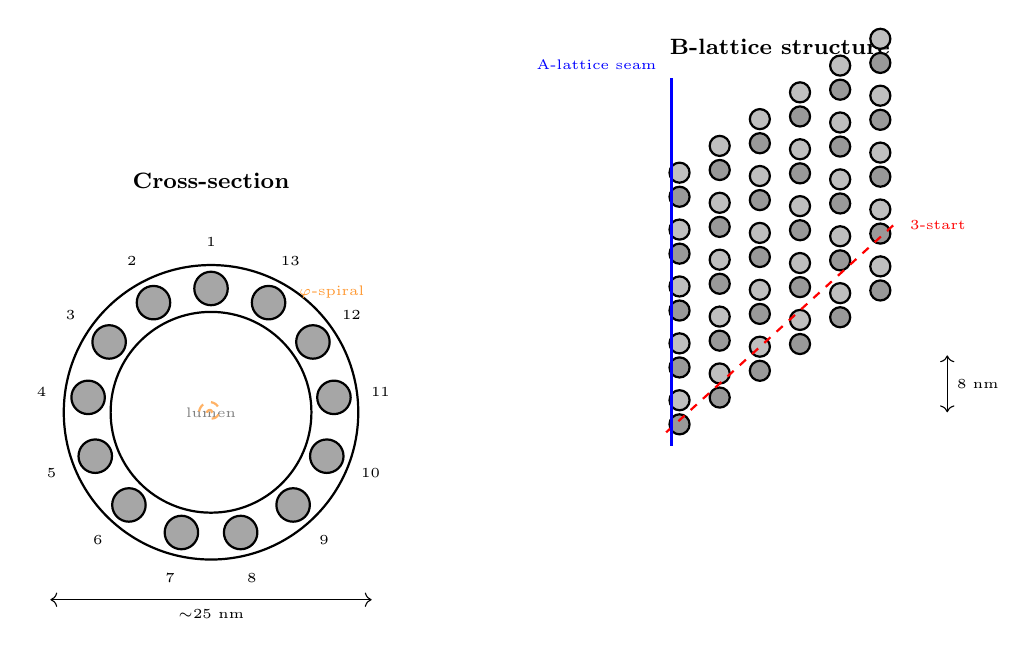
\begin{tikzpicture}[scale=0.85]
% === LEFT PANEL: Cross-section view ===
\begin{scope}[shift={(-4,0)}]
    \node[above,font=\footnotesize\bfseries] at (0,3.2) {Cross-section};
    \draw[thick] (0,0) circle (2.2);
    \draw[thick] (0,0) circle (1.5);
    \foreach \i in {1,...,13} {
        \pgfmathsetmacro{\angle}{90 + (\i-1)*360/13}
        \fill[gray!70] (\angle:1.85) circle (0.25);
        \draw[thick] (\angle:1.85) circle (0.25);
        \node[font=\tiny] at (\angle:2.55) {\i};
    }
    \node[font=\tiny,gray] at (0,0) {lumen};
    \draw[<->,thin] (-2.4,-2.8) -- (2.4,-2.8);
    \node[below,font=\tiny] at (0,-2.8) {$\sim$25 nm};
    \draw[orange!60,thick,dashed,domain=0:540,samples=150,smooth]
        plot ({0.06*\x/180*cos(\x)},{0.06*\x/180*sin(\x)});
    \node[orange!80,font=\tiny] at (1.8,1.8) {$\gr$-spiral};
\end{scope}
% === RIGHT PANEL: Longitudinal/unrolled lattice view ===
\begin{scope}[shift={(3,0)}]
    \node[above,font=\footnotesize\bfseries] at (1.5,5.2) {B-lattice structure};
    \foreach \col in {0,...,5} {
        \foreach \row in {0,...,4} {
            \pgfmathsetmacro{\yoff}{\col*0.4}
            \pgfmathsetmacro{\xpos}{\col*0.6}
            \pgfmathsetmacro{\ypos}{\row*0.85 + \yoff}
            \fill[gray!50] (\xpos,\ypos+0.18) circle (0.15);
            \draw[thick] (\xpos,\ypos+0.18) circle (0.15);
            \fill[gray!80] (\xpos,\ypos-0.18) circle (0.15);
            \draw[thick] (\xpos,\ypos-0.18) circle (0.15);
        }
    }
    \draw[red,thick,dashed] (-0.2,-0.3) -- (3.2,2.8);
    \node[red,font=\tiny,right] at (3.3,2.8) {3-start};
    \draw[blue,very thick] (-0.12,-0.5) -- (-0.12,5);
    \node[blue,font=\tiny,left] at (-0.2,5.2) {A-lattice seam};
    \draw[<->,thin] (4,0) -- (4,0.85);
    \node[right,font=\tiny] at (4,0.42) {8 nm};
\end{scope}
\end{tikzpicture}
\caption{\textbf{Microtubule lattice architecture establishes the geometric foundation for $\gr$-scaling.} \textit{Left:} Cross-section showing 13 protofilaments arranged cylindrically; the $\gr$-spiral overlay indicates the geometric relationship underlying eigenmode scaling. \textit{Right:} Unrolled B-lattice with $\alpha$-tubulin (light) and $\beta$-tubulin (dark) dimers. The 3-start helical pitch (red dashed) and A-lattice seam (blue) break cylindrical symmetry, introducing geometric phase for propagating modes and enabling topological protection of quantum coherence. \emph{Illustrative schematic for conceptual orientation; not drawn to molecular scale.}}
\label{fig:microtubule_geometry}
\end{figure}

%------------------------------------------------------------------------------
\subsection{$\pi$-Electron Systems in Tubulin}
\label{subsec:pi_electrons}
%------------------------------------------------------------------------------

Each tubulin monomer contains aromatic amino acid residues---tryptophan, tyrosine, phenylalanine---whose conjugated ring systems support delocalized $\pi$-electron clouds \citep{Craddock2017}. These electrons occupy molecular orbitals extending over multiple atoms, exhibiting quantum mechanical properties including superposition, tunneling, and entanglement.

The electronic Hamiltonian follows the extended Hubbard model:
\begin{equation}
\hat{H}_{\pi} = \sum_i \epsilon_i \hat{c}_i^\dagger \hat{c}_i + \sum_{\langle i,j \rangle} t_{ij} \left(\hat{c}_i^\dagger \hat{c}_j + \text{h.c.}\right) + \sum_{i < j} \frac{V_{ij}}{r_{ij}} \hat{n}_i \hat{n}_j
\label{eq:pi_hamiltonian}
\end{equation}
where $\epsilon_i$ denotes on-site energies, $t_{ij} \sim 0.1$--$1$~eV are hopping integrals, $V_{ij}$ captures Coulomb interactions, and $\hat{c}_i^\dagger$, $\hat{c}_i$, $\hat{n}_i$ are creation, annihilation, and number operators respectively.

Each tubulin monomer contains approximately 4 tryptophans, 5 tyrosines, and 8 phenylalanines, creating a distributed network capable of quantum coherent energy transfer analogous to photosynthetic systems \citep{Engel2007}.

%------------------------------------------------------------------------------
\subsection{Fr\"{o}hlich Coherence}
\label{subsec:frohlich}
%------------------------------------------------------------------------------

\citet{Frohlich1968} proposed that biological systems can sustain coherent vibrational modes through metabolic energy pumping. Energy input from GTP hydrolysis excites high-frequency modes, which condense into a coherent state:
\begin{equation}
\langle n_k \rangle = \frac{1}{\exp\left[(\hbar\omega_k - \mu_{\text{eff}})/k_B T_{\text{eff}}\right] - 1}
\label{eq:frohlich_distribution}
\end{equation}
where $\mu_{\text{eff}}$ is the effective chemical potential from metabolic pumping and $T_{\text{eff}} < T_{\text{physical}}$ when pumping exceeds dissipation.

When pumping rate exceeds a critical threshold, the lowest-frequency mode accumulates macroscopic occupation---a ``Fr\"{o}hlich condensate'' exhibiting long-range phase coherence. Terahertz spectroscopy has revealed resonant absorption in microtubules at predicted frequencies \citep{Sahu2013}.

%------------------------------------------------------------------------------
\subsection{Objective Reduction}
\label{subsec:orch_or}
%------------------------------------------------------------------------------

Penrose's objective reduction hypothesis\footnote{In this paper, `reduction' refers to the Penrose gravitational threshold condition; the subsequent dynamical evolution is provided by the VFD resonance-boundary framework.} derives from the incompatibility between quantum superposition and general relativistic spacetime geometry \citep{Penrose1996}. A mass in superposition creates superposed spacetime geometries---a fundamentally unstable configuration.

The transition timescale is:
\begin{equation}
\taucol = \frac{\hbar}{\EG}
\label{eq:penrose_time}
\end{equation}
where the gravitational self-energy is:
\begin{equation}
\EG = \frac{G}{c^2} \iint \frac{[\rho(\mathbf{r}) - \rho'(\mathbf{r})][\rho(\mathbf{r}') - \rho'(\mathbf{r}')]}{|\mathbf{r} - \mathbf{r}'|} \, d^3r \, d^3r'
\label{eq:gravitational_self_energy}
\end{equation}

For $N$ entangled tubulins, collective self-energy scales as $\EG^{(N)} \sim N^2 \cdot \EG^{(1)}$, yielding $\taucol^{(N)} \sim \taucol^{(1)}/N^2$. For $N \sim 10^{10}$ tubulins, $\taucol^{(N)} \sim 25$~ms---consistent with the temporal grain of conscious experience \citep{Hameroff2014}.

%------------------------------------------------------------------------------
\subsection{VFD Core Structures}
\label{subsec:vfd_foundations}
%------------------------------------------------------------------------------

Vibrational Field Dynamics provides the geometric-resonance framework organizing coherence across scales. Three core structures underpin the formalism:

\textbf{1. $\gr$-Scaled Resonance Hierarchy}: Coherence domains whose frequencies relate by powers of the golden ratio:
\begin{equation}
\gr = \frac{1 + \sqrt{5}}{2} \approx 1.618034
\label{eq:golden_ratio}
\end{equation}
For fundamental frequency $f_0$:
\begin{equation}
f_n = f_0 \cdot \gr^n, \quad n \in \mathbb{Z}
\label{eq:phi_scaling}
\end{equation}

\textbf{2. Torsional Field Operator}:
\begin{equation}
\hat{\Tfield}(\mathbf{r}, t) = \sum_n A_n \, e^{i(k_n \cdot \mathbf{r} - \omega_n t + \phi_n)} \hat{\sigma}_n
\label{eq:torsion_operator}
\end{equation}
where $\hat{\sigma}_n$ are generalized Pauli operators on the $n$-th resonance shell.

\textbf{3. Coherence Field}:
\begin{equation}
\Cfield(\mathbf{r}, t) = \left| \left\langle \prod_n e^{i\phi_n(\mathbf{r}, t)} \right\rangle \right|^2 \in [0, 1]
\label{eq:coherence_field}
\end{equation}
where $\Cfield = 1$ represents perfect phase-locking and $\Cfield = 0$ complete decoherence. Conscious states require $\Cfield > \Ccrit$ across multiple $\gr$-resonance shells.

\emph{With these foundations established, we now turn to the quantum origin layer where consciousness emerges.}

\vspace{0.5em}
\noindent\textbf{Methodological note:} The mechanisms proposed in the following sections represent a candidate unification pathway between Orch-OR and VFD. They do not claim to solve consciousness, nor to conclusively establish microtubule quantum coherence. The framework is exploratory and intended to support further empirical and theoretical investigation.

%==============================================================================
\section{The Quantum Origin Layer}
\label{sec:quantum_origin}
%==============================================================================

The quantum substrate of consciousness begins with $\pi$-electron dynamics in tubulin aromatic systems. This section traces the pathway from electronic wavefunctions through metabolic driving to the lattice boundary conditions that generate $\gr$-scaled eigenmodes.

%------------------------------------------------------------------------------
\subsection{$\pi$-Electron Wavefunctions}
\label{subsec:pi_wavefunctions}
%------------------------------------------------------------------------------

In the H\"{u}ckel approximation, $\pi$-electron wavefunctions take the form:
\begin{equation}
\Psi_n(\mathbf{r}) = \sum_{j=1}^{N_{\text{ring}}} c_{nj} \, \phi_j(\mathbf{r})
\label{eq:huckel_wavefunction}
\end{equation}
where $\phi_j$ are $2p_z$ atomic orbitals and coefficients $c_{nj}$ satisfy the secular equation $\det(\mathbf{H} - E\mathbf{S}) = 0$.

The aromatic systems---tryptophan (indole, 9 atoms), tyrosine (phenol, 7 atoms), phenylalanine (benzene, 6 atoms)---support delocalized wavefunctions with energy spacings $\Delta E \sim 1$--$4$~eV.

%------------------------------------------------------------------------------
\subsection{Metabolic Driving}
\label{subsec:superposition}
%------------------------------------------------------------------------------

Under metabolic driving from GTP hydrolysis:
\begin{equation}
\hat{H}(t) = \hat{H}_0 + \hat{V}_0 \cos(\omega_d t)
\label{eq:driven_hamiltonian}
\end{equation}
Resonance occurs when $\omega_d \approx (E_m - E_n)/\hbar$. Within the VFD framework, optimal coherence maintenance occurs when driving frequencies conform to $\gr$-ratios with natural transition frequencies, creating constructive interference that extends coherence lifetimes \citep{Cao2020}.

%------------------------------------------------------------------------------
\subsection{Dipole Coupling}
\label{subsec:dipole_coupling}
%------------------------------------------------------------------------------

Aromatic systems interact through transition dipole coupling:
\begin{equation}
V_{12} = \frac{1}{4\pi\epsilon_0} \left[ \frac{\boldsymbol{\mu}_1 \cdot \boldsymbol{\mu}_2}{R^3} - \frac{3(\boldsymbol{\mu}_1 \cdot \hat{\mathbf{R}})(\boldsymbol{\mu}_2 \cdot \hat{\mathbf{R}})}{R^3} \right]
\label{eq:dipole_coupling}
\end{equation}
Coherent energy transfer requires $|V_{12}| > \hbar \gamma_{\text{deco}}$, where $\gamma_{\text{deco}}$ is the decoherence rate. For tubulin aromatics with $|\boldsymbol{\mu}| \sim 5$~Debye and $R \sim 1$--$2$~nm, $V_{12} \sim 10$--$100$~cm$^{-1}$, comparable to photosynthetic complexes \citep{Engel2007, Craddock2017}.

%------------------------------------------------------------------------------
\subsection{Lattice Boundary Conditions}
\label{subsec:lattice_boundary}
%------------------------------------------------------------------------------

The microtubule cylinder imposes boundary conditions on quantum wavefunctions:
\begin{equation}
\Psi(r, \theta + 2\pi, z) = \Psi(r, \theta, z) \cdot e^{i\Phi_{\text{helix}}}
\label{eq:helical_boundary}
\end{equation}
where $\Phi_{\text{helix}} = 2\pi \times 3/13 \approx 1.451$~rad.

This quantizes angular momentum:
\begin{equation}
L_z = \hbar \left( m + \frac{3}{13} \right), \quad m \in \mathbb{Z}
\label{eq:angular_momentum_quantization}
\end{equation}
The A-lattice seam introduces additional phase matching that couples modes with different $m$, enabling topological protection.

\emph{These boundary conditions, arising directly from microtubule geometry, generate the $\gr$-scaled eigenmode spectrum derived in the following section.}

%==============================================================================
\section{Microtubule Lattice Eigenmodes}
\label{sec:lattice_eigenmodes}
%==============================================================================

This section presents the central mathematical result: the derivation of $\gr$-scaled eigenfrequencies from microtubule lattice geometry. This geometric origin---rather than \emph{ad hoc} assumption---provides the physical grounding absent in previous formulations.

%------------------------------------------------------------------------------
\subsection{Vibrational Spectrum}
\label{subsec:vibrational_modes}
%------------------------------------------------------------------------------

The microtubule supports vibrational modes satisfying the Helmholtz equation:
\begin{equation}
\left( \nabla^2 + k_{mnl}^2 \right) \Psi_{mnl}(r, \theta, z) = 0
\label{eq:helmholtz}
\end{equation}
with eigenfrequencies:
\begin{equation}
\omega_{mnl} = c_{\text{eff}} \sqrt{\left(\frac{\alpha_{mn}}{a}\right)^2 + \left(\frac{m}{a}\right)^2 + \left(\frac{l\pi}{L}\right)^2}
\label{eq:eigenfrequencies}
\end{equation}
where $a \approx 12.5$~nm is the cylinder radius, $L$ is length, $c_{\text{eff}} = \sqrt{E/\rho}$ with Young's modulus $E \sim 1$~GPa and density $\rho \sim 1500$~kg/m$^3$, and $\alpha_{mn}$ are Bessel function zeros.

For the 13-protofilament structure with 3-start helix:
\begin{equation}
\omega_n = \omega_0 \sqrt{1 + \left( \frac{3n}{13} \right)^2}, \quad n = 0, \pm 1, \pm 2, \ldots
\label{eq:helical_frequencies}
\end{equation}

%------------------------------------------------------------------------------
\subsection{Torsional Modes and $\gr$-Scaling}
\label{subsec:torsional_modes}
%------------------------------------------------------------------------------

Torsional oscillations about the cylinder axis satisfy the wave equation:
\begin{equation}
\frac{\partial^2 \phi}{\partial t^2} = c_t^2 \frac{\partial^2 \phi}{\partial z^2}
\label{eq:torsional_wave}
\end{equation}
with torsional wave speed $c_t = \sqrt{G_{\text{shear}}/\rho} \approx 500$~m/s, yielding:
\begin{equation}
f_n^{\text{tors}} = \frac{n \, c_t}{2L}, \quad n = 1, 2, 3, \ldots
\label{eq:torsional_frequencies}
\end{equation}

\textbf{Key Result}: For microtubule lengths $L_m = L_0 \cdot \gr^m$ (with $L_0 \approx 1~\mu$m), consecutive eigenfrequencies approach:
\begin{equation}
\boxed{\frac{f_{n+1}^{\text{tors}}}{f_n^{\text{tors}}} \to \gr \quad \text{as } n \to \infty}
\label{eq:phi_scaling_torsion}
\end{equation}
This result suggests neuronal microtubules may be length-regulated to optimize $\gr$-resonance---a testable prediction (Section~\ref{subsec:pred5}).

%------------------------------------------------------------------------------
\subsection{Topological Protection via Seam Geometry}
\label{subsec:seam_topology}
%------------------------------------------------------------------------------

The A-lattice seam introduces a topological defect analogous to a screw dislocation. A wavefunction encircling the seam acquires geometric (Berry) phase:
\begin{equation}
\gamma_{\text{seam}} = \oint_C \mathbf{A}_{\text{eff}} \cdot d\mathbf{l} = \frac{2\pi \times 3}{13} \approx 1.451~\text{rad}
\label{eq:seam_phase}
\end{equation}
where $\mathbf{A}_{\text{eff}}$ is the effective gauge connection.

This provides \emph{topological protection}: perturbations that do not alter seam topology cannot decohere phase-protected modes \citep{Berry1984, Kitaev2003}. We propose this as a candidate mechanism for biological decoherence protection, subject to experimental verification.

%------------------------------------------------------------------------------
\subsection{Complete Eigenmode Hierarchy}
\label{subsec:phi_eigenmodes}
%------------------------------------------------------------------------------

The complete spectrum combining axial, circumferential, and radial modes is:
\begin{equation}
f_{nml}^{\text{MT}} = f_0 \sqrt{n^2 + \left(\frac{3m}{13}\right)^2 + \alpha_{\text{rad}} l^2}
\label{eq:full_spectrum}
\end{equation}
where $n, m, l$ are axial, circumferential, and radial quantum numbers respectively, and $\alpha_{\text{rad}}$ is a geometric factor. This expression is schematic and captures the qualitative structure of the spectrum; exact numerical predictions for specific microtubules require detailed molecular dynamics simulations.

The fundamental frequency:
\begin{equation}
f_0^{\text{MT}} \approx \frac{c_{\text{eff}}}{2L} \sim 8.3~\text{MHz}
\label{eq:fundamental_frequency}
\end{equation}
for $L = 3~\mu$m, $c_{\text{eff}} = 50$~m/s, establishes the base of the $\gr$-ladder connecting quantum to macroscopic scales. Here $c_{\text{eff}}$ denotes an effective longitudinal wave speed incorporating internal damping, boundary conditions, and complex viscoelastic interactions, which reduce the usable propagation speed far below $\sqrt{E/\rho}$.

% FIGURE 2: Phi-Scaled Eigenmodes
\begin{figure}[htbp]
\centering
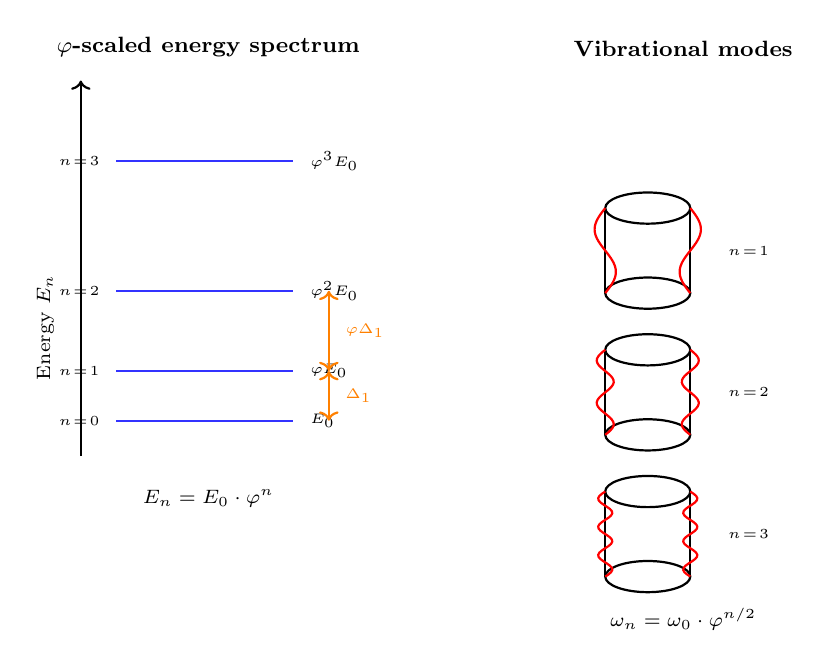
\begin{tikzpicture}[scale=0.9]
% === LEFT PANEL: Energy Level Diagram ===
\begin{scope}[shift={(-4,0)}]
    \node[above,font=\footnotesize\bfseries] at (1.8,5.5) {$\gr$-scaled energy spectrum};
    \draw[->,thick] (0,0) -- (0,5.3);
    \node[left,font=\scriptsize,rotate=90] at (-0.5,2.7) {Energy $E_n$};
    \pgfmathsetmacro{\escale}{0.7}
    \pgfmathsetmacro{\Ezero}{0.5}
    \draw[thick,blue!80] (0.5,\Ezero) -- (3,\Ezero);
    \node[left,font=\tiny] at (0.4,\Ezero) {$n\!=\!0$};
    \node[right,font=\tiny] at (3.1,\Ezero) {$E_0$};
    \pgfmathsetmacro{\Eone}{0.5 + 0.7*1}
    \draw[thick,blue!80] (0.5,\Eone) -- (3,\Eone);
    \node[left,font=\tiny] at (0.4,\Eone) {$n\!=\!1$};
    \node[right,font=\tiny] at (3.1,\Eone) {$\gr E_0$};
    \pgfmathsetmacro{\Etwo}{0.5 + 0.7*2.618}
    \draw[thick,blue!80] (0.5,\Etwo) -- (3,\Etwo);
    \node[left,font=\tiny] at (0.4,\Etwo) {$n\!=\!2$};
    \node[right,font=\tiny] at (3.1,\Etwo) {$\gr^2 E_0$};
    \pgfmathsetmacro{\Ethree}{0.5 + 0.7*5.236}
    \draw[thick,blue!80] (0.5,\Ethree) -- (3,\Ethree);
    \node[left,font=\tiny] at (0.4,\Ethree) {$n\!=\!3$};
    \node[right,font=\tiny] at (3.1,\Ethree) {$\gr^3 E_0$};
    \draw[<->,orange,thick] (3.5,\Ezero) -- (3.5,\Eone);
    \node[right,font=\tiny,orange] at (3.6,{(\Ezero+\Eone)/2}) {$\Delta_1$};
    \draw[<->,orange,thick] (3.5,\Eone) -- (3.5,\Etwo);
    \node[right,font=\tiny,orange] at (3.6,{(\Eone+\Etwo)/2}) {$\gr\Delta_1$};
    \node[font=\scriptsize] at (1.8,-0.6) {$E_n = E_0 \cdot \gr^n$};
\end{scope}
% === RIGHT PANEL: Mode shapes on cylinder ===
\begin{scope}[shift={(4,0)}]
    \node[above,font=\footnotesize\bfseries] at (0.5,5.5) {Vibrational modes};
    \begin{scope}[shift={(0,3.5)}]
        \draw[thick] (0,0) ellipse (0.6 and 0.22);
        \draw[thick] (-0.6,0) -- (-0.6,-1.2);
        \draw[thick] (0.6,0) -- (0.6,-1.2);
        \draw[thick] (0,-1.2) ellipse (0.6 and 0.22);
        \draw[red,thick,domain=0:1.2,samples=40] plot ({0.6+0.15*sin(360*\x/1.2)},{-\x});
        \draw[red,thick,domain=0:1.2,samples=40] plot ({-0.6-0.15*sin(360*\x/1.2)},{-\x});
        \node[right,font=\tiny] at (1,-0.6) {$n\!=\!1$};
    \end{scope}
    \begin{scope}[shift={(0,1.5)}]
        \draw[thick] (0,0) ellipse (0.6 and 0.22);
        \draw[thick] (-0.6,0) -- (-0.6,-1.2);
        \draw[thick] (0.6,0) -- (0.6,-1.2);
        \draw[thick] (0,-1.2) ellipse (0.6 and 0.22);
        \draw[red,thick,domain=0:1.2,samples=40] plot ({0.6+0.12*sin(720*\x/1.2)},{-\x});
        \draw[red,thick,domain=0:1.2,samples=40] plot ({-0.6-0.12*sin(720*\x/1.2)},{-\x});
        \node[right,font=\tiny] at (1,-0.6) {$n\!=\!2$};
    \end{scope}
    \begin{scope}[shift={(0,-0.5)}]
        \draw[thick] (0,0) ellipse (0.6 and 0.22);
        \draw[thick] (-0.6,0) -- (-0.6,-1.2);
        \draw[thick] (0.6,0) -- (0.6,-1.2);
        \draw[thick] (0,-1.2) ellipse (0.6 and 0.22);
        \draw[red,thick,domain=0:1.2,samples=40] plot ({0.6+0.1*sin(1080*\x/1.2)},{-\x});
        \draw[red,thick,domain=0:1.2,samples=40] plot ({-0.6-0.1*sin(1080*\x/1.2)},{-\x});
        \node[right,font=\tiny] at (1,-0.6) {$n\!=\!3$};
    \end{scope}
    \node[font=\scriptsize] at (0.5,-2.3) {$\omega_n = \omega_0 \cdot \gr^{n/2}$};
\end{scope}
\end{tikzpicture}
\caption{\textbf{$\gr$-scaled eigenmode spectrum (illustrative) may provide decoherence protection through frequency niche separation.} \textit{Left:} Energy levels with golden ratio spacing $E_n = E_0 \gr^n$. The irrational (maximally non-resonant) spacing minimizes coupling to integer-harmonic thermal noise. \textit{Right:} Corresponding vibrational mode shapes on cylindrical microtubule geometry, with increasing node number for higher modes. This candidate mechanism requires experimental verification. \emph{Illustrative schematic for conceptual orientation; not representing literal mode shapes.}}
\label{fig:phi_eigenmodes}
\end{figure}

\emph{The $\gr$-scaled spectrum established here (Figure~\ref{fig:phi_eigenmodes}) provides the foundation for the dual transition criterion developed in the following section. With the geometric origin of the eigenmode hierarchy now established, we turn to the central question: how do quantum state transitions occur within this resonance architecture, and what role does the VFD coherence field play in determining transition outcomes?}

%==============================================================================
\section{The Transition Mechanism: VFD Reinterpretation}
\label{sec:collapse_mechanism}
%==============================================================================

This section presents the central theoretical innovation: reinterpretation of objective reduction as a \emph{resonance-boundary transition} (RBT)\footnote{RBT refers to the proposed VFD-compatible dynamical transition in microtubule quantum states that preserves Penrose's OR threshold while adding a geometric resonance-selection mechanism.} requiring \emph{both} Penrose gravitational threshold \emph{and} VFD coherence boundary transition. Penrose OR is retained as a gravitational instability threshold, but the physical transition itself is not a classical wavefunction collapse. Instead, within VFD the transition is a resonance-boundary transition into the next $\gr$-stable coherent state. This preserves Penrose's gravitational criterion while eliminating metaphysical collapse language. The dual criterion resolves the timing problem and provides the missing link between quantum events and conscious experience.

%------------------------------------------------------------------------------
\subsection{Standard Orch-OR Transition}
\label{subsec:standard_orchor}
%------------------------------------------------------------------------------

In Orch-OR, tubulin dimers exist in quantum superposition:
\begin{equation}
|\psi\rangle_{\text{tubulin}} = \alpha |0\rangle + \beta |1\rangle, \quad |\alpha|^2 + |\beta|^2 = 1
\label{eq:tubulin_qubit}
\end{equation}
where $|0\rangle$ and $|1\rangle$ represent conformations differing by mass displacement $\delta x \sim 0.1$~nm.

Entanglement creates collective superposition:
\begin{equation}
|\Psi\rangle_N = \frac{1}{\sqrt{2}} \left( |0\rangle^{\otimes N} + |1\rangle^{\otimes N} \right)
\label{eq:entangled_state}
\end{equation}
The resonance-boundary transition occurs when gravitational self-energy reaches threshold, with timescale given by Eq.~\eqref{eq:penrose_time}.

%------------------------------------------------------------------------------
\subsection{VFD Reinterpretation: Resonance Boundary Transition}
\label{subsec:vfd_collapse}
%------------------------------------------------------------------------------

VFD provides a complementary interpretation: objective reduction represents a \emph{resonance-boundary transition} (RBT) within the coherence field.

The coherence field evolves according to:
\begin{equation}
\frac{\partial \Cfield}{\partial t} = D_{\Cfield} \nabla^2 \Cfield + \lambda \Cfield (1 - \Cfield) - \gamma \Cfield + S(\mathbf{r}, t)
\label{eq:coherence_evolution}
\end{equation}
where $D_{\Cfield}$ is the diffusion coefficient, $\lambda$ is the self-amplification rate, $\gamma$ is the decoherence rate, and $S$ represents metabolic driving. We present this PDE as a minimal phenomenological form intended to illustrate the proposed mechanism; quantitative parameter values require experimental determination.

This equation exhibits \emph{bistability}: stable solutions at $\Cfield \approx 1$ (high coherence) and $\Cfield \approx 0$ (decoherent), with sharp transition at critical threshold $\Ccrit$.

The \textbf{unified transition criterion} combines both requirements:
\begin{equation}
\boxed{\Gamma_{\text{transition}} = \frac{\EG}{\hbar} \cdot \Theta(\Cfield - \Ccrit)}
\label{eq:dual_collapse}
\end{equation}
where $\Theta$ is the Heaviside step function. The resonance-boundary transition occurs \emph{only when both} gravitational threshold \emph{and} coherence boundary conditions are satisfied.

We present this dual criterion as a candidate mechanism within the unified VFD--Orch-OR framework, subject to future empirical investigation.

Within this unified framework, Penrose OR is not interpreted as a literal destruction of the wavefunction, but as the moment when gravitational self-energy instabilities force the quantum--geometric system to undergo a resonance-boundary transition. The system does not ``collapse'' in the classical sense; rather, it transitions into the next $\gr$-stable coherent state permitted by the underlying $\gr$-resonance shell geometry. This preserves Penrose's gravitational criterion while providing the missing dynamical mechanism through VFD.

\textbf{Key clarification}: Penrose's gravitational threshold remains fully intact and unchanged in this formulation. VFD contributes only the dynamical boundary-selection mechanism that determines \emph{which} coherent state the system transitions into. The proposed reinterpretation preserves all Orch-OR physics and adds a geometric layer specifying the post-transition stable states.

\emph{Clarification}: This formulation retains Penrose's core reasoning and threshold condition exactly. The gravitational instability triggers the transition; the VFD coherence field determines the final stable state. VFD supplies an extended dynamical context, not a replacement for OR.

% FIGURE 4: Dual Transition Criterion
\begin{figure}[htbp]
\centering
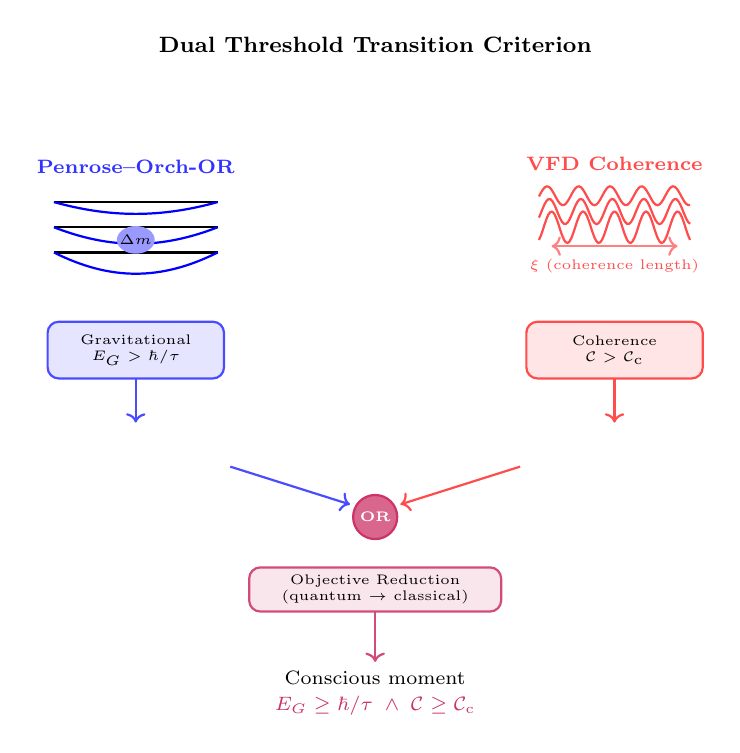
\begin{tikzpicture}[scale=0.8]
\node[font=\footnotesize\bfseries] at (0,5.5) {Dual Threshold Transition Criterion};
% === LEFT PATH: Penrose Gravitational ===
\begin{scope}[shift={(-3.8,0)}]
    \draw[thick] (-1.3,3) -- (1.3,3);
    \draw[thick] (-1.3,2.6) -- (1.3,2.6);
    \draw[thick] (-1.3,2.2) -- (1.3,2.2);
    \draw[thick,blue] (-1.3,3) .. controls (-0.4,2.75) and (0.4,2.75) .. (1.3,3);
    \draw[thick,blue] (-1.3,2.6) .. controls (-0.4,2.25) and (0.4,2.25) .. (1.3,2.6);
    \draw[thick,blue] (-1.3,2.2) .. controls (-0.4,1.75) and (0.4,1.75) .. (1.3,2.2);
    \fill[blue!40] (0,2.4) ellipse (0.3 and 0.22);
    \node[font=\tiny] at (0,2.4) {$\Delta m$};
    \node[above,font=\scriptsize\bfseries,blue!80] at (0,3.3) {Penrose--Orch-OR};
    \draw[thick,blue!70,fill=blue!10,rounded corners] (-1.4,0.2) rectangle (1.4,1.1);
    \node[font=\tiny,align=center] at (0,0.65) {Gravitational\\$\EG > \hbar/\taucol$};
    \draw[->,thick,blue!70] (0,0.2) -- (0,-0.5);
\end{scope}
% === RIGHT PATH: VFD Coherence ===
\begin{scope}[shift={(3.8,0)}]
    \draw[thick,red!70,domain=-1.2:1.2,samples=80] plot (\x,{2.6+0.25*cos(720*\x)});
    \draw[thick,red!70,domain=-1.2:1.2,samples=80] plot (\x,{2.85+0.2*cos(720*\x+25)});
    \draw[thick,red!70,domain=-1.2:1.2,samples=80] plot (\x,{3.1+0.15*cos(720*\x+50)});
    \draw[<->,red!50,thick] (-1,2.3) -- (1,2.3);
    \node[below,font=\tiny,red!70] at (0,2.25) {$\xi$ (coherence length)};
    \node[above,font=\scriptsize\bfseries,red!70] at (0,3.35) {VFD Coherence};
    \draw[thick,red!70,fill=red!10,rounded corners] (-1.4,0.2) rectangle (1.4,1.1);
    \node[font=\tiny,align=center] at (0,0.65) {Coherence\\$\Cfield > \Ccrit$};
    \draw[->,thick,red!70] (0,0.2) -- (0,-0.5);
\end{scope}
% === CONVERGENCE ZONE ===
\begin{scope}[shift={(0,-1.8)}]
    \draw[->,thick,blue!70] (-2.3,0.6) -- (-0.4,0);
    \draw[->,thick,red!70] (2.3,0.6) -- (0.4,0);
    \fill[purple!60] (0,-0.2) circle (0.35);
    \draw[thick,purple!80] (0,-0.2) circle (0.35);
    \node[white,font=\tiny\bfseries] at (0,-0.2) {OR};
    \draw[thick,purple!70,fill=purple!10,rounded corners] (-2,-1.7) rectangle (2,-1);
    \node[font=\tiny,align=center] at (0,-1.35) {Objective Reduction\\(quantum $\to$ classical)};
    \draw[->,thick,purple!70] (0,-1.7) -- (0,-2.5);
    \node[below,font=\scriptsize] at (0,-2.5) {Conscious moment};
\end{scope}
\node[font=\scriptsize,purple!80] at (0,-5) {$\EG \geq \hbar/\taucol \;\wedge\; \Cfield \geq \Ccrit$};
\end{tikzpicture}
\caption{\textbf{Dual transition criterion (schematic) illustrates proposed timing specificity of conscious experience.} Objective reduction requires \emph{both} Penrose gravitational threshold ($\EG > \hbar/\taucol$, left pathway) \emph{and} VFD coherence threshold ($\Cfield > \Ccrit$, right pathway). This dual requirement ensures resonance-boundary transitions correlate with coherent conscious state rather than occurring at arbitrary intervals---resolving a key challenge for Orch-OR. \emph{Illustrative schematic for conceptual orientation; exact values remain to be determined experimentally.}}
\label{fig:dual_collapse}
\end{figure}

%------------------------------------------------------------------------------
\subsection{Resolution of Orch-OR Challenges}
\label{subsec:challenge_resolution}
%------------------------------------------------------------------------------

The unified framework (Figure~\ref{fig:dual_collapse}) addresses each challenge identified in Section~\ref{sec:introduction}:

\textbf{1. Decoherence Protection}: The $\gr$-hierarchy creates frequency niches where thermal noise has minimal spectral overlap:
\begin{equation}
\langle n_{\text{noise}}(\omegagr) \rangle \ll \langle n_{\text{noise}}(\omega_{\text{random}}) \rangle
\label{eq:noise_mismatch}
\end{equation}
Seam topology provides additional topological protection via Berry phase (Eq.~\ref{eq:seam_phase}).

\textbf{2. Scale Bridging}: The $\gr$-ladder provides mathematical continuity:
\begin{equation}
f^{\text{MT}} \cdot \gr^{-N} = f^{\text{cortex}}, \quad N \approx 12\text{--}15
\label{eq:scale_bridge}
\end{equation}

\textbf{3. Timing Specificity}: The dual criterion explains why resonance-boundary transitions correlate with conscious state---both thresholds must be satisfied simultaneously.

\textbf{4. Bidirectional Causation}: Macroscopic fields modulate $\Cfield$ boundary conditions (developed in Section~\ref{sec:top_down}).

\textbf{5. Phenomenal Binding}: Global phase-locking ($\Cfield \to 1$) provides a physical basis for unified experience.

\emph{Having established the transition mechanism, we now examine its relationship to fundamental limits of computation. The resonance-boundary transition framework raises a deeper question: in what sense does VFD operate outside the domain of conventional algorithmic processes, and how does this relate to Penrose's arguments about consciousness and computability?}

%==============================================================================
\section{Beyond Turing: Continuous Geometric Computation in VFD}
\label{sec:beyond_turing}
%==============================================================================

This section establishes a crucial conceptual foundation: the relationship between Turing computation, physical dynamics, and the geometric architecture of VFD. We demonstrate that VFD operates in a continuous geometric regime that \emph{embeds} discrete symbolic computation as a limiting case, providing a mathematical framework in which non-computable physical processes may support consciousness.

%------------------------------------------------------------------------------
\subsection{Turing Computation as Discrete Symbol Manipulation}
\label{subsec:turing_limits}
%------------------------------------------------------------------------------

A Turing machine manipulates finite symbolic states according to deterministic rules, reading and writing discrete symbols on an infinite tape \citep{Turing1936}. This model captures the essence of algorithmic computation and underlies all digital computers. However, it is essential to recognise that Turing computation is a \emph{model of discrete symbol manipulation}, not a physical law. Uncomputability in the Turing sense is a limitation of symbolic formalisms, not a limitation of physical law.

Physics, by contrast, is fundamentally continuous, geometric, and field-based. The evolution of physical systems---whether electromagnetic fields, fluid flows, or quantum wavefunctions---occurs in continuous state spaces governed by differential equations rather than discrete symbolic updates.

This observation carries a crucial implication: the halting problem and related undecidability results apply to discrete formal systems, not to continuous geometric fields. These limitations are therefore \emph{epistemic}---properties of the representational formalism---not \emph{ontological} properties of the physical world.

The uncomputability discussed here is epistemic rather than ontological: it pertains to the limitations of discrete symbolic models, not of physical law. This argument does not imply humans, brains, or consciousness violate Turing computation; rather, it highlights that physical dynamics often operate in a continuous geometric domain larger than discrete computation frameworks. The purpose of this section is to position VFD within that continuous domain, not to assert metaphysical claims about intelligence or computability.

This distinction has significant implications. For nearly a century, an implicit assumption has pervaded theoretical discourse: that computation, symbolic manipulation, Turing machines, and physical simulation are essentially equivalent. Yet continuous geometric systems need not conform to this equivalence. The limitations identified by Turing constrain the class of discrete symbolic machines that attempt to \emph{represent} physical evolution---they do not constrain the geometric field evolution itself.

%------------------------------------------------------------------------------
\subsection{Non-Computable Behaviour in Physical Systems}
\label{subsec:noncomputable_physics}
%------------------------------------------------------------------------------

Recent mathematical developments provide rigorous support for this distinction. \citet{Miranda2025} demonstrated that continuous physical systems---specifically, solutions to the Euler equations governing ideal fluid flow---can exhibit behaviour that is formally uncomputable by any Turing machine. This result extends earlier work showing undecidability in dynamical systems \citep{Moore1990, daCosta1991} and confirms that uncomputability is not confined to exotic quantum-gravitational regimes but emerges in ordinary classical physics.

Physical systems can evolve in ways that no algorithmic machine can fully predict, yet their geometry remains lawful and structured. Crucially, the presence of Turing-uncomputable behaviour does not imply randomness, unpredictability, or mystical processes. Rather, it indicates that physical evolution in continuous geometric spaces cannot always be fully represented by discrete symbolic machines:

\begin{quote}
\emph{Uncomputability is not a property of the universe; it is a property of the discrete symbolic machines used to describe the universe.}
\end{quote}

Physics remains lawful even where Turing computation cannot fully capture it.

This distinction supports Penrose's thesis that consciousness may require non-computable physics \citep{Penrose1989, Penrose1994}. The recognition that non-computable behaviour appears in ordinary physical systems---not merely in speculative quantum-gravitational scenarios---broadens the empirical basis for this view. The demonstration that even classical fluid dynamics can exhibit Turing-uncomputable behaviour suggests that continuous physical systems naturally operate in a regime broader than discrete symbolic computation.

\textbf{Important clarification}: This does not imply that biological systems violate the Church--Turing thesis. Rather, it highlights that continuous geometric dynamics are not confined to discrete symbolic computation, and therefore exceed classical computational descriptions while remaining fully physical. The Church--Turing thesis concerns the class of functions computable by algorithmic means; it does not assert that all physical processes are algorithmically simulable.

%------------------------------------------------------------------------------
\subsection{VFD as Continuous Harmonic Field Geometry}
\label{subsec:vfd_geometry}
%------------------------------------------------------------------------------

VFD extends computation beyond the Turing domain by working in continuous, geometric, harmonic manifolds. Discrete computation becomes a special case of constrained VFD dynamics. Rather than discrete symbolic states, VFD models physics through $\gr$-scaled resonance manifolds---smooth, continuous, topological structures whose evolution is governed by geometric constraints rather than discrete symbolic updates.

In VFD, the coherence field $\Cfield(\mathbf{r}, t)$ evolves on a continuous manifold according to:
\begin{equation}
\frac{\partial \Cfield}{\partial t} = \mathcal{F}[\Cfield, \nabla\Cfield, \nabla^2\Cfield; \gr]
\label{eq:vfd_continuous}
\end{equation}
where $\mathcal{F}$ is a nonlinear functional incorporating $\gr$-scaled coupling between resonance shells. This illustrative expression captures the essential continuous character of VFD evolution; it occurs in an infinite-dimensional function space, not a finite discrete state space.

Uncomputability in the Turing sense does not imply physical unpredictability; it indicates instead that discrete symbolic machines cannot capture the evolution of continuous geometric fields. The limitations of Turing computation reflect the limitations of the representational formalism, not of the physics itself. The $\gr$-scaled harmonic geometry of VFD operates precisely in this non-discrete regime, offering a continuous-field description where `uncomputable' behaviour becomes structured and lawful. Thus, uncomputability is not an obstacle to a physical theory of consciousness---it is evidence that a geometric framework such as VFD is required.

VFD operates outside the Turing domain because it is: (i)~\emph{continuous} rather than discrete; (ii)~\emph{geometric} rather than symbolic; (iii)~\emph{harmonic} rather than algorithmic; (iv)~\emph{scale-linked} through $\gr$-ratios rather than level-separated; and (v)~\emph{resonance-based} rather than rule-based. These properties place VFD in a broader geometric regime that contains discrete computation as a special case.

%------------------------------------------------------------------------------
\subsection{Turing Computation as a Special Case of VFD}
\label{subsec:turing_special_case}
%------------------------------------------------------------------------------

A key insight of this framework is that VFD does not reject Turing computation---it \emph{embeds} it. Turing computation emerges as a special limiting case when the continuous VFD field is restricted to a finite set of stable attractor basins.

Consider a coherence field with $N$ discrete stable attractors $\{\Cfield_1, \Cfield_2, \ldots, \Cfield_N\}$ separated by energy barriers. When the field is confined to transitions between these attractors, its dynamics reduce to:
\begin{equation}
\Cfield(t) \in \{\Cfield_1, \ldots, \Cfield_N\}, \quad \Cfield(t+\Delta t) = T[\Cfield(t), I(t)]
\label{eq:discrete_limit}
\end{equation}
where $T$ is a transition function and $I(t)$ represents input. This is precisely a finite-state machine---the core of Turing computation.

Symbolic state transitions correspond to transitions between these attractors, mediated by perturbations that push the field over energy barriers. In this restricted regime, the continuous field dynamics collapse to discrete symbolic manipulation. Therefore:

\begin{quote}
\emph{In VFD, computation emerges as geometric evolution in a continuous field. Turing-style computation corresponds to the highly restricted case where the coherence field is forced into discrete, bistable attractor states.}
\end{quote}

This embedding relationship clarifies the scope of each framework:
\begin{itemize}
    \item \textbf{Turing domain}: Discrete attractors, symbolic transitions, algorithmic processing
    \item \textbf{VFD domain}: Continuous manifolds, geometric evolution, harmonic resonance
    \item \textbf{Relationship}: Turing $\subset$ VFD (proper subset)
\end{itemize}

%------------------------------------------------------------------------------
\subsection{Implications for Consciousness and Artificial Systems}
\label{subsec:consciousness_ai}
%------------------------------------------------------------------------------

Within the present framework, the distinction between Turing and geometric computation has immediate implications for understanding consciousness:

\begin{enumerate}
    \item \textbf{Orch-OR provides the microphysical substrate}: Penrose's objective reduction introduces a fundamentally non-computable state-selection mechanism at the quantum-gravitational interface.

    \item \textbf{VFD provides the geometric propagation architecture}: The $\gr$-scaled harmonic field carries non-computable effects coherently upward through microtubules, cellular networks, and cortical harmonics to global consciousness.

    \item \textbf{Turing uncomputability reinforces the necessity of geometric frameworks}: Discrete symbolic computation cannot capture the continuous, harmonic, scale-linked resonance dynamics central to VFD.
\end{enumerate}

This framework also clarifies the relationship between biological consciousness and artificial computation. Current artificial systems operate within the Turing-subset of VFD's geometric hierarchy: discrete, symbol-based, algorithmic processing. Biological consciousness, by contrast, may arise in the continuous, resonance-driven domain that lies outside the discrete symbolic regime. This distinction is mathematical, grounded in the geometry of the coherence field.

\emph{Caveat}: This suggests---but does not prove---that geometric, continuous, resonance-based processes may be necessary for conscious dynamics. The framework provides a candidate mechanism, not a definitive solution to the consciousness problem.

\emph{Having established the computational framework and its relationship to uncomputability, we now trace how quantum events propagate upward through biological scales. The continuous geometric domain described above must connect to specific biological structures; the following section maps this $\gr$-resonance architecture onto the nested hierarchy of neural organization from $\pi$-electrons to cortical dynamics.}

%==============================================================================
\section{Upscaling Through Biological Levels}
\label{sec:upscaling}
%==============================================================================

The $\gr$-ladder connects quantum events to macroscopic cognition through successive levels of biological organization. This section traces the pathway from $\pi$-electrons through tubulin dimers, protofilaments, neural networks, to cortical dynamics.

%------------------------------------------------------------------------------
\subsection{$\pi$-Electron to Tubulin Dimer}
\label{subsec:electron_to_dimer}
%------------------------------------------------------------------------------

When the Born-Oppenheimer approximation breaks down, electronic and nuclear degrees of freedom become entangled:
\begin{equation}
|\Psi\rangle = \sum_n \chi_n(\mathbf{R}) \otimes |\psi_n^{\text{elec}}(\mathbf{r}; \mathbf{R})\rangle
\label{eq:entangled_electron_nuclear}
\end{equation}
where $\chi_n(\mathbf{R})$ are nuclear wavefunctions and $|\psi_n^{\text{elec}}\rangle$ are electronic states parametrically dependent on nuclear coordinates $\mathbf{R}$.

Conformational changes inherit quantum superposition from $\pi$-electrons, making the tubulin dimer a mesoscopic quantum system capable of participating in collective coherence.

%------------------------------------------------------------------------------
\subsection{Protofilament to Network}
\label{subsec:protofilament_network}
%------------------------------------------------------------------------------

Within protofilaments, dimers couple through a Bose-Hubbard-type Hamiltonian:
\begin{equation}
\hat{H}_{\text{chain}} = \sum_i \epsilon_i \hat{n}_i + \sum_{\langle ij \rangle} J_{ij} (\hat{a}_i^\dagger \hat{a}_j + \text{h.c.}) + \sum_i \frac{U_i}{2} \hat{n}_i(\hat{n}_i - 1)
\label{eq:protofilament_hamiltonian}
\end{equation}
where $\epsilon_i$ are on-site energies, $J_{ij}$ are hopping integrals, and $U_i$ is the on-site interaction.

Collective modes propagate as Bloch waves with dispersion:
\begin{equation}
\omega(k) = \sqrt{\epsilon_0^2 + 4J^2 \sin^2(ka/2)}
\label{eq:dispersion}
\end{equation}

%------------------------------------------------------------------------------
\subsection{Neural Network: Kuramoto Synchronization}
\label{subsec:kuramoto}
%------------------------------------------------------------------------------

At the network level, oscillators couple through Kuramoto dynamics:
\begin{equation}
\frac{d\theta_i}{dt} = \omega_i + \sum_j K_{ij} \sin(\theta_j - \theta_i)
\label{eq:kuramoto}
\end{equation}
where $\theta_i$ is the phase of oscillator $i$, $\omega_i$ is its natural frequency, and $K_{ij}$ is the coupling strength.

The order parameter $r e^{i\psi} = N^{-1} \sum_j e^{i\theta_j}$ measures global synchronization. VFD predicts quantum-enhanced correlations yield:
\begin{equation}
r_{\text{quantum}} > r_{\text{classical}}
\label{eq:enhanced_synchronization}
\end{equation}
manifesting as enhanced gamma coherence during conscious states \citep{Fries2015, Singer1999}.

%------------------------------------------------------------------------------
\subsection{Cortical Harmonics}
\label{subsec:cortical_harmonics}
%------------------------------------------------------------------------------

Cortical oscillations form standing waves satisfying the Helmholtz equation on the cortical surface \citep{Atasoy2016}:
\begin{equation}
\nabla^2 \Phi + k^2 \Phi = 0
\label{eq:cortical_helmholtz}
\end{equation}

VFD predicts optimal frequencies follow $\gr$-scaling, connecting microtubule to cortical dynamics:
\begin{equation}
f^{\text{MT}} = f^{\text{cortex}} \cdot \gr^N, \quad N \sim 12\text{--}15
\label{eq:complete_ladder}
\end{equation}
This completes the resonance ladder spanning 15 orders of magnitude from quantum ($\sim$THz) to cortical ($\sim$Hz) frequencies. Figure~\ref{fig:resonance_shells} illustrates this $\gr$-resonance shell hierarchy and its scaling relationship across nested anatomical and energetic levels.

% FIGURE 4: Multi-Scale Resonance Shell Hierarchy
\begin{figure}[htbp]
\centering
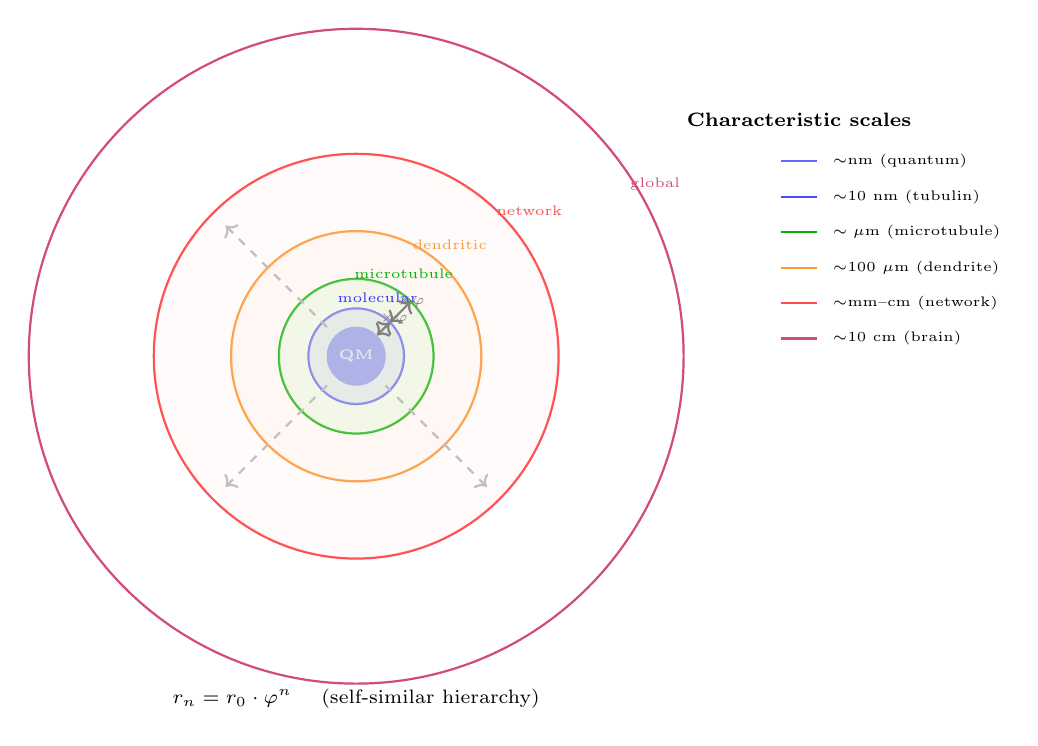
\begin{tikzpicture}[scale=0.75]
\fill[blue!60,opacity=0.8] (0,0) circle (0.5);
\node[white,font=\tiny\bfseries] at (0,0) {QM};
\pgfmathsetmacro{\rone}{0.5*1.618}
\draw[thick,blue!70] (0,0) circle (\rone);
\fill[blue!30,opacity=0.25] (0,0) circle (\rone);
\pgfmathsetmacro{\rtwo}{0.5*1.618*1.618}
\draw[thick,green!70!black] (0,0) circle (\rtwo);
\fill[green!30,opacity=0.2] (0,0) circle (\rtwo);
\pgfmathsetmacro{\rthree}{0.5*1.618*1.618*1.618}
\draw[thick,orange!80] (0,0) circle (\rthree);
\fill[orange!20,opacity=0.15] (0,0) circle (\rthree);
\pgfmathsetmacro{\rfour}{0.5*1.618*1.618*1.618*1.618}
\draw[thick,red!70] (0,0) circle (\rfour);
\fill[red!15,opacity=0.1] (0,0) circle (\rfour);
\pgfmathsetmacro{\rfive}{0.5*1.618*1.618*1.618*1.618*1.618}
\draw[thick,purple!70] (0,0) circle (\rfive);
\node[font=\tiny,blue!80] at (70:\rone+0.25) {molecular};
\node[font=\tiny,green!70!black] at (60:\rtwo+0.3) {microtubule};
\node[font=\tiny,orange!80] at (50:\rthree+0.35) {dendritic};
\node[font=\tiny,red!70] at (40:\rfour+0.4) {network};
\node[font=\tiny,purple!70] at (30:\rfive+0.3) {global};
\begin{scope}[shift={(7.5,1.5)}]
    \node[font=\scriptsize\bfseries] at (0,2.5) {Characteristic scales};
    \draw[blue!60,thick] (-0.3,1.8) -- (0.3,1.8);
    \node[right,font=\tiny] at (0.4,1.8) {$\sim$nm (quantum)};
    \draw[blue!70,thick] (-0.3,1.2) -- (0.3,1.2);
    \node[right,font=\tiny] at (0.4,1.2) {$\sim$10 nm (tubulin)};
    \draw[green!70!black,thick] (-0.3,0.6) -- (0.3,0.6);
    \node[right,font=\tiny] at (0.4,0.6) {$\sim\mu$m (microtubule)};
    \draw[orange!80,thick] (-0.3,0) -- (0.3,0);
    \node[right,font=\tiny] at (0.4,0) {$\sim$100 $\mu$m (dendrite)};
    \draw[red!70,thick] (-0.3,-0.6) -- (0.3,-0.6);
    \node[right,font=\tiny] at (0.4,-0.6) {$\sim$mm--cm (network)};
    \draw[purple!70,thick] (-0.3,-1.2) -- (0.3,-1.2);
    \node[right,font=\tiny] at (0.4,-1.2) {$\sim$10 cm (brain)};
\end{scope}
\draw[<->,thick,gray] (45:0.5) -- (45:\rone);
\node[gray,font=\tiny] at (45:{0.5+(\rone-0.5)/2+0.25}) {$\times\gr$};
\draw[<->,thick,gray] (45:\rone) -- (45:\rtwo);
\node[gray,font=\tiny] at (45:{\rone+(\rtwo-\rone)/2+0.25}) {$\times\gr$};
\foreach \angle in {135,225,315} {
    \draw[->,thick,gray!50,dashed] (\angle:0.7) -- (\angle:\rfour-0.3);
}
\node[font=\scriptsize] at (0,-5.8) {$r_n = r_0 \cdot \gr^n$ \quad (self-similar hierarchy)};
\end{tikzpicture}
\caption{\textbf{VFD $\gr$-resonance shell hierarchy (schematic) proposes a solution to the scale-bridging problem.} Concentric $\gr$-scaled shells connect quantum ($\sim$nm) through cellular ($\sim\mu$m) to cortical ($\sim$cm) scales. Each shell radius relates to adjacent shells by the golden ratio, creating mathematical continuity across 15 orders of magnitude. Dashed arrows indicate proposed resonance coupling enabling coherent information transfer between scales. \emph{Illustrative schematic for conceptual orientation; not drawn to scale.}}
\label{fig:resonance_shells}
\end{figure}

\emph{The upscaling pathway established here enables bidirectional causation, developed formally in Section~\ref{sec:top_down}.}

%==============================================================================
\section{VFD Formalism}
\label{sec:vfd_unification}
%==============================================================================

This section develops the mathematical formalism of Vibrational Field Dynamics, providing the rigorous foundation for the unified theory.

%------------------------------------------------------------------------------
\subsection{$\gr$-Resonance Shell Structure}
\label{subsec:phi_shells}
%------------------------------------------------------------------------------

Each resonance shell responds to frequencies near its characteristic value according to:
\begin{equation}
\Sfield_n(\omega) = \exp\left[ -\frac{(\omega - \omega_0 \gr^n)^2}{2\sigma_n^2} \right]
\label{eq:shell_function}
\end{equation}
where $\sigma_n$ is the shell bandwidth, typically $\sigma_n \sim \omega_0 \gr^n / Q$ with quality factor $Q \sim 10$--$100$.

Total coherence integrating across shells:
\begin{equation}
\Cfield_{\text{total}} = \sum_n w_n \cdot \Cfield_n \cdot \prod_{m \neq n} F_{nm}(\Delta\phi_{nm})
\label{eq:total_coherence}
\end{equation}
where $w_n$ are shell weights, $\Cfield_n$ is the coherence within shell $n$, and $F_{nm}$ are inter-shell coupling functions depending on phase differences $\Delta\phi_{nm}$. This illustrative form captures the hierarchical coupling structure; the precise functional dependence requires empirical determination.

The $\gr$-ratio ensures optimal phase relationships through the Fibonacci limit:
\begin{equation}
\gr = \lim_{n \to \infty} \frac{F_{n+1}}{F_n}
\label{eq:fibonacci_limit}
\end{equation}
where $F_n$ are Fibonacci numbers. This mathematical relationship ensures $\gr$-scaled frequencies avoid destructive resonance while maintaining connectedness (see Appendix~\ref{app:phi_derivation}).

%------------------------------------------------------------------------------
\subsection{Braid Operators}
\label{subsec:torsional_braids}
%------------------------------------------------------------------------------

VFD introduces braid operators $\hat{\Bfield}_i$ for topological phase relationships:
\begin{equation}
\hat{\Bfield}_i = \exp\left[ i\frac{\pi}{4} \left(\hat{\sigma}_z^{(i)} \otimes \hat{\sigma}_z^{(i+1)}\right) \right]
\label{eq:braid_generator}
\end{equation}
satisfying the Yang-Baxter equation:
\begin{equation}
\hat{\Bfield}_i \hat{\Bfield}_{i+1} \hat{\Bfield}_i = \hat{\Bfield}_{i+1} \hat{\Bfield}_i \hat{\Bfield}_{i+1}
\label{eq:yang_baxter}
\end{equation}

The microtubule seam naturally implements braid operations as helical waves traverse the structure, providing a physical substrate for topologically-protected quantum computation.

%------------------------------------------------------------------------------
\subsection{Coherence Field Dynamics}
\label{subsec:coherence_dynamics}
%------------------------------------------------------------------------------

The complete coherence field equation is:
\begin{equation}
\frac{\partial \Cfield}{\partial t} = D_{\Cfield} \nabla^2 \Cfield + f(\Cfield) - \gamma \Cfield + I_{\text{ext}}
\label{eq:brain_coherence}
\end{equation}
with bistable nonlinearity:
\begin{equation}
f(\Cfield) = \lambda \Cfield (1 - \Cfield)(\Cfield - \Ccrit)
\label{eq:bistable_nonlinearity}
\end{equation}
This phenomenological form captures the essential bistable dynamics; specific functional forms and parameter values remain to be determined experimentally.

Conscious states require coherence exceeding critical threshold throughout the conscious domain $\Omega_{\text{conscious}}$:
\begin{equation}
\Cfield(\mathbf{r}, t) > \Ccrit \quad \forall \, \mathbf{r} \in \Omega_{\text{conscious}}
\label{eq:conscious_threshold}
\end{equation}

Phenomenal binding arises from global phase-locking:
\begin{equation}
\left| \langle e^{i(\phi_i - \phi_j)} \rangle \right| \approx 1 \quad \forall \, i, j \in \Omega_{\text{conscious}}
\label{eq:phase_locking}
\end{equation}
We present this as a candidate mechanism for phenomenal unity, subject to future empirical investigation.

%==============================================================================
\section{Bidirectional Causation}
\label{sec:top_down}
%==============================================================================

A central challenge for any physical theory of consciousness is explaining how macroscopic mental states (attention, intention) can influence microscopic processes. This section demonstrates how VFD enables bidirectional causation through coherence field modulation.

%------------------------------------------------------------------------------
\subsection{Attention as Field Modulation}
\label{subsec:attention}
%------------------------------------------------------------------------------

Attention corresponds to spatially-selective modulation of the coherence field:
\begin{equation}
\Cfield(\mathbf{r}, t) \to \Cfield(\mathbf{r}, t) \cdot A(\mathbf{r}, t)
\label{eq:attention_modulation}
\end{equation}
where $A(\mathbf{r}, t)$ is the attention field with $A > 1$ in attended regions.

This propagates through the $\gr$-hierarchy via convolution:
\begin{equation}
A^{(n)}(\mathbf{r}, t) = \int G_n(\mathbf{r} - \mathbf{r}') A^{(n+1)}(\mathbf{r}', t) \, d^3r'
\label{eq:attention_cascade}
\end{equation}
where $G_n$ is the Green's function for shell $n$.

At the microtubule level, attention modifies inter-dimer coupling:
\begin{equation}
J_{ij} \to J_{ij} + \delta J_{ij}^{\text{att}}
\label{eq:coupling_modulation}
\end{equation}

%------------------------------------------------------------------------------
\subsection{Intention and Transition Bias}
\label{subsec:intention}
%------------------------------------------------------------------------------

Conscious intention generates coherent field patterns:
\begin{equation}
I(\mathbf{r}, t) = I_0 \cdot \Phi_{\text{intent}}(\mathbf{r}) \cdot e^{i\omega_I t}
\label{eq:intention_field}
\end{equation}
where $\Phi_{\text{intent}}$ encodes the spatial structure of the intended action.

These patterns modulate quantum boundary conditions:
\begin{equation}
\left. \Psi \right|_{\partial\Omega_{\text{MT}}} = \Psi_0 \cdot [1 + \epsilon \cdot I(\mathbf{r}, t)]
\label{eq:boundary_modulation}
\end{equation}

Yielding biased transition probabilities:
\begin{equation}
P(|0\rangle) - P(|1\rangle) = \Delta P \propto \epsilon \cdot |I|
\label{eq:biased_probability}
\end{equation}

This does \emph{not} violate quantum mechanics: the Born rule is preserved locally. State \emph{preparation} through macroscopic field effects creates a feedback loop enabling physical top-down causation without introducing new physics.

%------------------------------------------------------------------------------
\subsection{Coupled Macro-Micro Dynamics}
\label{subsec:top_down_math}
%------------------------------------------------------------------------------

The complete coupled system:
\begin{align}
\frac{d\Cfield^{\text{macro}}}{dt} &= F[\Cfield^{\text{macro}}, \langle\hat{O}\rangle^{\text{micro}}] + I_{\text{ext}} \label{eq:macro_evolution} \\
i\hbar \frac{\partial |\Psi^{\text{micro}}\rangle}{\partial t} &= \hat{H}[\Cfield^{\text{macro}}] |\Psi^{\text{micro}}\rangle \label{eq:micro_evolution}
\end{align}

The macro equation depends on quantum expectation values; the micro equation has a Hamiltonian parametrically dependent on the macroscopic field. This creates the bidirectional coupling illustrated in Figure~\ref{fig:macro_micro}.

Transition probability density incorporating both criteria:
\begin{equation}
\rho_{\text{transition}}(\mathbf{x}, t) = |\Psi(\mathbf{x})|^2 \cdot \Theta[\Cfield(\mathbf{x}) - \Ccrit] \cdot \delta(\EG - \EG^{\text{crit}})
\label{eq:collapse_density}
\end{equation}

% FIGURE 5: Macro-Micro Bidirectional Causation
\begin{figure}[htbp]
\centering
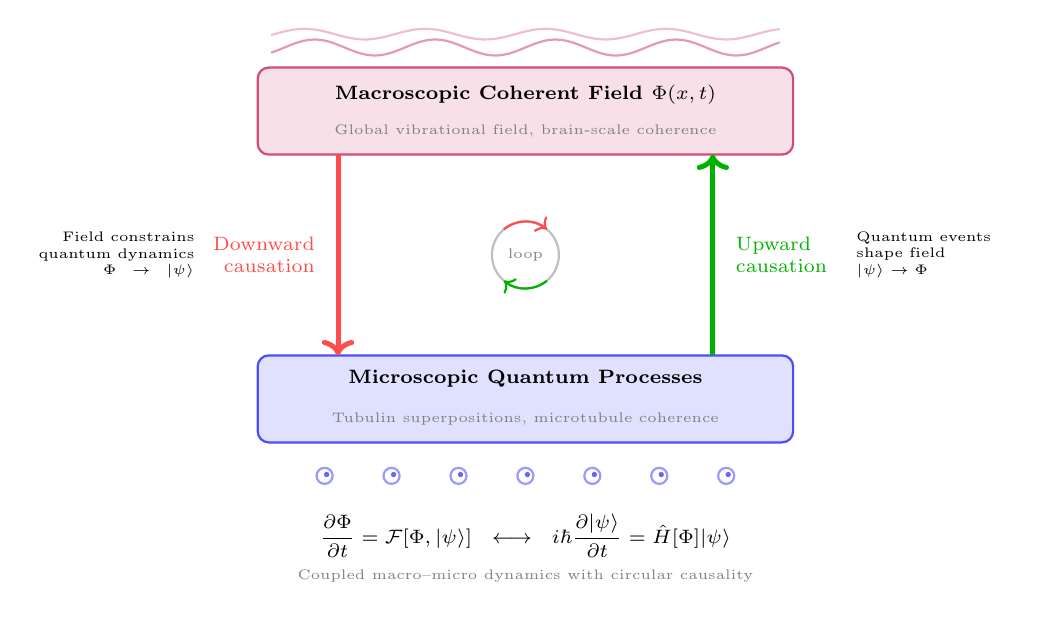
\begin{tikzpicture}[scale=0.85]
\draw[thick,purple!70,fill=purple!12,rounded corners] (-4,3.5) rectangle (4,4.8);
\node[font=\scriptsize\bfseries] at (0,4.4) {Macroscopic Coherent Field $\Phi(x,t)$};
\node[font=\tiny,gray] at (0,3.85) {Global vibrational field, brain-scale coherence};
\draw[purple!40,thick,domain=-3.8:3.8,samples=80] plot (\x,{5.1+0.12*sin(200*\x)});
\draw[purple!25,thick,domain=-3.8:3.8,samples=80] plot (\x,{5.3+0.08*sin(200*\x+30)});
\draw[thick,blue!70,fill=blue!12,rounded corners] (-4,-0.8) rectangle (4,0.5);
\node[font=\scriptsize\bfseries] at (0,0.15) {Microscopic Quantum Processes};
\node[font=\tiny,gray] at (0,-0.45) {Tubulin superpositions, microtubule coherence};
\foreach \x in {-3,-2,-1,0,1,2,3} {
    \draw[blue!40,thick] (\x,-1.3) circle (0.12);
    \fill[blue!60] (\x,-1.3) ++(0.03,0.02) circle (0.04);
}
\draw[->,very thick,red!70,line width=1.8pt] (-2.8,3.5) -- (-2.8,0.5);
\node[left,font=\scriptsize,red!70,align=right] at (-3,2) {Downward\\causation};
\node[left,font=\tiny,text width=2cm,align=right] at (-4.8,2) {Field constrains\\quantum dynamics\\$\Phi \to |\psi\rangle$};
\draw[->,very thick,green!70!black,line width=1.8pt] (2.8,0.5) -- (2.8,3.5);
\node[right,font=\scriptsize,green!70!black,align=left] at (3,2) {Upward\\causation};
\node[right,font=\tiny,text width=2cm,align=left] at (4.8,2) {Quantum events\\shape field\\$|\psi\rangle \to \Phi$};
\begin{scope}[shift={(0,2)}]
    \draw[thick,gray!50] (0,0) circle (0.5);
    \draw[->,red!70,thick] (130:0.5) arc (130:50:0.5);
    \draw[->,green!70!black,thick] (-50:0.5) arc (-50:-130:0.5);
    \node[font=\tiny,gray] at (0,0) {loop};
\end{scope}
\node[font=\scriptsize] at (0,-2.2) {%
    $\displaystyle \frac{\partial \Phi}{\partial t} = \mathcal{F}[\Phi, |\psi\rangle]$
    \;\;$\longleftrightarrow$\;\;
    $\displaystyle i\hbar\frac{\partial |\psi\rangle}{\partial t} = \hat{H}[\Phi]|\psi\rangle$};
\node[font=\tiny,gray] at (0,-2.8) {Coupled macro--micro dynamics with circular causality};
\end{tikzpicture}
\caption{\textbf{Bidirectional causation (schematic) proposes how mental causation may be grounded in explicit physics.} Macroscopic mental states (attention, intention) modulate the coherence field $\Cfield$, which propagates downward through the $\gr$-resonance shell hierarchy to influence quantum boundary conditions (red arrow). Conversely, quantum resonance-boundary transition events propagate upward to shape macroscopic field dynamics (green arrow). This circular causality operates through the coupled equations~\eqref{eq:macro_evolution}--\eqref{eq:micro_evolution} without violating quantum mechanics. \emph{Illustrative schematic for conceptual orientation; coupling mechanisms shown are candidate proposals subject to experimental investigation.}}
\label{fig:macro_micro}
\end{figure}

\emph{The bidirectional causation framework established above completes the mechanistic picture: quantum events influence macroscopic dynamics, while macroscopic states constrain quantum evolution. With all components now in place---quantum substrate, lattice eigenmodes, transition mechanism, computational framework, biological upscaling, field formalism, and causal architecture---we can synthesize these into a unified theoretical structure.}

%==============================================================================
\section{Unified Theory: Complete Synthesis}
\label{sec:unified_theory}
%==============================================================================

This section synthesizes the preceding developments into a coherent theoretical framework, stating core principles, defining the state space, and presenting the variational formulation.

%------------------------------------------------------------------------------
\subsection{Core Principles}
\label{subsec:core_principles}
%------------------------------------------------------------------------------

The unified VFD--Orch-OR theory rests on six principles:

\begin{description}
    \item[P1. Quantum Substrate:] Consciousness has its physical basis in quantum superposition of $\pi$-electron states in neuronal microtubules.

    \item[P2. Geometric Structure:] Microtubule lattice geometry---13 protofilaments, B-lattice configuration, A-lattice seam---establishes boundary conditions generating topologically-protected eigenmodes.

    \item[P3. $\gr$-Resonance:] Eigenmode frequencies follow $\gr$-scaling, creating an optimal hierarchy for coherence maintenance and cross-scale propagation.

    \item[P4. Dual Transition:] Objective reduction requires \emph{both} Penrose gravitational threshold \emph{and} VFD coherence boundary transition.

    \item[P5. Resonance Ladder:] Multi-scale coupling through $\gr$-frequencies connects quantum events to cortical dynamics across 15 orders of magnitude.

    \item[P6. Bidirectional Causation:] Macroscopic field states modulate microscopic boundary conditions, enabling top-down influence within physical law.
\end{description}

\textbf{Hierarchy of contributions}: Orch-OR provides the threshold event---the gravitational instability that triggers state transitions at the quantum-gravitational interface. VFD provides the continuous geometric substrate that propagates boundary-condition changes across biological scales through the $\gr$-hierarchy.

\textbf{Why the combination is necessary}: Neither framework alone suffices. Orch-OR specifies \emph{when} transitions occur (gravitational threshold) but not \emph{how} quantum events propagate upward to cognition. VFD specifies \emph{how} coherence propagates across scales but requires an external mechanism for state selection. Together, they form a complete theory: OR triggers transitions; VFD determines stable states and propagates effects.

%------------------------------------------------------------------------------
\subsection{State Space}
\label{subsec:state_space}
%------------------------------------------------------------------------------

Conscious states occupy a manifold defined by:
\begin{equation}
\mathcal{M} = \{ (\Psi^{\text{MT}}, \Cfield, \Phi^{\text{cortex}}) : \Cfield > \Ccrit, \, \nabla \times \Tfield \neq 0 \}
\label{eq:state_manifold}
\end{equation}

Different conscious modes correspond to distinct trajectories on this manifold:
\begin{itemize}
    \item \textbf{Focused attention}: localized high-$\Cfield$ region
    \item \textbf{Diffuse awareness}: distributed moderate-$\Cfield$
    \item \textbf{Flow states}: temporally stable high-$\Cfield$ trajectory
    \item \textbf{Altered states}: modified $\gr$-resonance shell structure
\end{itemize}

%------------------------------------------------------------------------------
\subsection{Lagrangian Formulation}
\label{subsec:lagrangian}
%------------------------------------------------------------------------------

The theory admits a variational principle:
\begin{equation}
\boxed{\delta \int \left[ \Lcal_{\text{QM}} + \Lcal_{\text{VFD}} + \Lcal_{\text{neural}} + \Lcal_{\text{coupling}} \right] dt = 0}
\label{eq:variational_principle}
\end{equation}
with component Lagrangians:
\begin{align}
\Lcal_{\text{QM}} &= \langle \Psi | i\hbar\partial_t - \hat{H}_{\text{MT}} | \Psi \rangle \label{eq:L_QM}\\
\Lcal_{\text{VFD}} &= \frac{1}{2}(\partial_t \Cfield)^2 - V[\Cfield] - \frac{D_{\Cfield}}{2}|\nabla\Cfield|^2 \label{eq:L_VFD}\\
\Lcal_{\text{coupling}} &= \lambda_1 \Cfield \cdot |\Psi|^2 + \lambda_2 \Cfield \cdot \Phi^{\text{cortex}} \label{eq:L_coupling}
\end{align}
where $\lambda_1, \lambda_2$ are coupling constants.

This formulation enables standard field-theoretic analysis including symmetries, conservation laws, and perturbative corrections.

%==============================================================================
\section{Predictions and Experimental Tests}
\label{sec:predictions}
%==============================================================================

The unified theory generates seven experimentally testable predictions distinguishing it from both standard Orch-OR and classical neuroscience. These predictions are not confirmation of the theory; they define the experimental programme required to evaluate it. Confirmation would provide strong evidence supporting the framework; falsification would require revision or rejection. The predictions below are stated as hypotheses to be tested, not as claims about what will be found.

%------------------------------------------------------------------------------
\subsection{Prediction 1: $\gr$-Scaled Eigenfrequencies}
\label{subsec:pred1}
%------------------------------------------------------------------------------

\textbf{Hypothesis}: Microtubule resonant frequencies cluster at $f_n = f_0 \cdot \gr^n$ with $f_0 \approx 8.3$~MHz.

\textbf{Predicted pattern to test}: 8.3, 13.4, 21.7, 35.1, 56.8, 91.9, 148.7~MHz, $\ldots$

\textbf{Experimental test}: High-resolution microwave/terahertz spectroscopy of purified neuronal microtubules, comparing resonance structure to non-neuronal microtubules.

\textbf{Technology status}: THz spectroscopy of biological samples is mature; preliminary microtubule resonance studies exist \citep{Sahu2013} but have not specifically tested $\gr$-scaling.

%------------------------------------------------------------------------------
\subsection{Prediction 2: Enhanced Decoherence Protection}
\label{subsec:pred2}
%------------------------------------------------------------------------------

\textbf{Hypothesis}: Quantum coherence persists longer at $\gr$-frequencies than at arbitrary frequencies (order-of-magnitude estimate):
\begin{equation}
T_2(\omegagr) / T_2(\omega_{\text{random}}) \sim 3\text{--}10
\label{eq:decoherence_enhancement}
\end{equation}

\textbf{Experimental test}: Pump-probe spectroscopy comparing coherence decay times at $\gr$-scaled versus arbitrary frequencies in microtubule preparations.

\textbf{Technology status}: Ultrafast spectroscopy techniques for measuring quantum coherence exist for photosynthetic systems; adaptation to microtubule preparations has not yet been attempted.

%------------------------------------------------------------------------------
\subsection{Prediction 3: $\gr$-Scaled Gamma Harmonics}
\label{subsec:pred3}
%------------------------------------------------------------------------------

\textbf{Hypothesis}: Conscious states exhibit enhanced power at $\gr$-related gamma frequencies rather than integer harmonics.

For fundamental $f_\gamma = 40$~Hz: enhanced at 64.7, 104.7, 169.4~Hz ($\gr$-scaled); \emph{not} enhanced at 80, 120, 160~Hz (integer-scaled).

\textbf{Experimental test}: High-density EEG/MEG spectral analysis during conscious versus unconscious processing, testing for $\gr$-harmonic versus integer-harmonic power distributions.

\textbf{Technology status}: High-density EEG/MEG systems and spectral analysis methods are widely available. Existing datasets could be reanalysed for $\gr$-scaling; to our knowledge, this specific analysis has not been performed.

%------------------------------------------------------------------------------
\subsection{Prediction 4: Attention-Modulated Microtubule Spectra}
\label{subsec:pred4}
%------------------------------------------------------------------------------

\textbf{Hypothesis}: Focused attention modifies microtubule vibrational spectra in attended cortical regions.

\textbf{Experimental test}: Combined attention paradigms with conformational-sensitive fluorescent tubulin probes, correlating spectral changes with attention allocation.

\textbf{Technology status}: Conformational-sensitive probes for microtubules are in development but not yet sufficiently sensitive for in vivo neural measurements. This represents a medium-term technological target.

%------------------------------------------------------------------------------
\subsection{Prediction 5: $\gr$-Ratio Length Regulation}
\label{subsec:pred5}
%------------------------------------------------------------------------------

\textbf{Hypothesis}: Neuronal microtubules are length-regulated to $\gr$-ratios: $L_n / L_m \approx \gr^{n-m}$.

\textbf{Experimental test}: Super-resolution microscopy of microtubule length distributions in neurons versus non-neuronal cells, testing for $\gr$-ratio clustering in neuronal populations.

\textbf{Technology status}: Super-resolution microscopy (STORM, PALM) can resolve individual microtubules; length distribution studies in neurons are feasible with existing technology.

%------------------------------------------------------------------------------
\subsection{Prediction 6: $\gr$-Periodic Microstate Transitions}
\label{subsec:pred6}
%------------------------------------------------------------------------------

\textbf{Hypothesis}: EEG microstate transition times follow $\gr$-periodic modulation.

\textbf{Experimental test}: Analysis of microstate sequence timing for $\gr$-related periodicity versus random or integer-harmonic patterns.

\textbf{Technology status}: EEG microstate analysis is an established method. Existing microstate timing data could be reanalysed for $\gr$-periodicity without new data collection.

%------------------------------------------------------------------------------
\subsection{Prediction 7: Anesthetic Disruption of $\gr$-Structure}
\label{subsec:pred7}
%------------------------------------------------------------------------------

\textbf{Hypothesis}: Anesthetics disrupt consciousness by shifting microtubule eigenfrequencies away from $\gr$-ratios.

\textbf{Experimental test}: Microtubule spectroscopy under varying anesthetic concentrations, correlating frequency-ratio deviation with loss of consciousness.

\textbf{Technology status}: Anesthetic effects on microtubule dynamics have been studied; coupling spectroscopy with anaesthesiology protocols is technically feasible with current methods.

%------------------------------------------------------------------------------
\subsection{Roadmap for Experimental Verification}
\label{subsec:experimental_roadmap}
%------------------------------------------------------------------------------

The predictions outlined above define a structured experimental programme. We briefly outline how verification could proceed using near-term experimental tools, organised by timescale and technical requirements.

\textbf{Immediate tests (current technology)}:
\begin{itemize}
    \item \emph{Microtubule resonance spectroscopy}: Terahertz time-domain spectroscopy and pump-probe techniques can detect vibrational modes in purified microtubule preparations. The key test is whether resonance peaks cluster at $\gr$-related frequency ratios rather than arbitrary or integer-harmonic patterns. Recent advances in THz spectroscopy of biological samples \citep{Sahu2013} provide the technical foundation.

    \item \emph{Anesthetic perturbation studies}: Systematic measurement of microtubule vibrational spectra under varying anesthetic concentrations (propofol, sevoflurane, ketamine) can test whether loss of consciousness correlates with disruption of $\gr$-ratio structure. This requires combining anaesthesiology protocols with high-resolution spectroscopy.

    \item \emph{Cortical harmonic analysis}: Reanalysis of existing high-density EEG and MEG datasets for $\gr$-scaled harmonic signatures in gamma-band activity. The prediction is enhanced power at 64.7, 104.7, 169.4~Hz rather than integer harmonics of 40~Hz. This analysis can be performed on archived data with appropriate spectral methods.
\end{itemize}

\textbf{Medium-term directions (5--10 year horizon)}:
\begin{itemize}
    \item \emph{Coherence-mapping techniques}: Development of optical or magnetic probes capable of detecting quantum coherence in neural tissue with spatial resolution sufficient to map coherence across the $\gr$-hierarchy. Nitrogen-vacancy centre magnetometry and advanced fluorescence techniques offer promising avenues.

    \item \emph{$\gr$-scaled frequency scanning}: Systematic perturbation of neural systems at $\gr$-scaled frequencies to test for resonance-enhanced effects on cognitive performance, attention, or state transitions. Transcranial alternating current stimulation (tACS) protocols could be adapted for this purpose.

    \item \emph{MT-specific quantum control tools}: Development of pharmacological or genetic tools that selectively modulate microtubule quantum properties without disrupting classical cytoskeletal function, enabling isolation of quantum-specific contributions to consciousness.
\end{itemize}

\textbf{Long-term implications}:
Successful validation of these predictions would support the hypothesis that consciousness arises through specific quantum-resonant architecture rather than classical computation alone. This would: (i)~redirect neuroscience toward microtubule-level mechanisms; (ii)~suggest new targets for disorders of consciousness; (iii)~provide candidate design principles for any future attempt to create artificial conscious systems; and (iv)~contribute to debates about the role of quantum mechanics in biology.

Failure to observe the predicted signatures would constrain the framework, requiring either modification of specific parameter values or reconsideration of foundational assumptions. Either outcome advances scientific understanding.

%==============================================================================
\section{Significance and Open Questions}
\label{sec:significance}
%==============================================================================

The unified VFD--Orch-OR framework carries implications across multiple domains and suggests directions for future research.

%------------------------------------------------------------------------------
\subsection{Implications}
\label{subsec:implications}
%------------------------------------------------------------------------------

\textbf{For neuroscience}: If validated, the framework would redirect consciousness research toward microtubule integrity, $\gr$-ratio structure in neural oscillations, and cross-frequency coupling as resonance hierarchy manifestation. It offers an explanation for why gamma oscillations are prominent in conscious processing---they may represent the cortical terminus of the $\gr$-ladder \citep{Fries2015, Canolty2010}.

\textbf{For quantum biology}: VFD proposes specific decoherence protection mechanisms---frequency niche separation, topological protection via seam geometry, active metabolic maintenance---potentially extending quantum biology beyond photosynthesis \citep{Engel2007, Cao2020} to neural information processing.

\textbf{For philosophy of mind}: The theory offers a novel position: not dualist (all components physical), not eliminativist (phenomenal properties correspond to coherence field structure), not panpsychist (consciousness requires specific $\gr$-resonant architecture). Explicit mechanisms replace mysterious emergence.

\textbf{For artificial systems}: Current artificial systems operate within the Turing-subset of VFD's geometric hierarchy---discrete, symbol-based, algorithmic processing. If consciousness requires $\gr$-scaled quantum-resonant architecture, achieving artificial consciousness would require moving beyond classical digital computation to quantum substrates with appropriate geometric structure.

%------------------------------------------------------------------------------
\subsection{Open Research Directions}
\label{subsec:open_questions}
%------------------------------------------------------------------------------

Several questions remain for future investigation:

\begin{enumerate}
    \item \textbf{Quantitative parameter determination}: What are the precise values of coupling constants $\lambda_1, \lambda_2$, critical coherence $\Ccrit$, and shell quality factors $Q_n$?

    \item \textbf{Developmental emergence}: How does the $\gr$-architecture develop during neural maturation? Is it genetically specified or self-organizing?

    \item \textbf{Pathological disruption}: Do disorders of consciousness (anesthesia, coma, psychosis) correspond to specific disruptions of $\gr$-structure?

    \item \textbf{Inter-species variation}: Does the framework predict consciousness gradations across species based on microtubule architecture?

    \item \textbf{Integration with bioelectricity}: How does VFD relate to other field-theoretic approaches to biological organization and developmental bioelectricity?
\end{enumerate}

These questions define a research program that could be pursued through collaborative efforts across quantum physics, neuroscience, and consciousness studies.

\emph{The significance of this framework lies not merely in its theoretical coherence but in its capacity to generate testable predictions and guide experimental research. We now summarise the central contributions and their implications.}

%==============================================================================
\section{Conclusion}
\label{sec:conclusion}
%==============================================================================

We have presented a unified theoretical framework integrating Orchestrated Objective Reduction with Vibrational Field Dynamics. The central contribution is proposing that VFD may provide the geometric-resonance architecture needed to transform Orch-OR from an isolated quantum hypothesis into a complete, multi-scale physical theory.

The framework proposes:
\begin{enumerate}
    \item $\pi$-electron quantum superposition in tubulin aromatics provides the quantum substrate

    \item Microtubule lattice geometry generates topologically-protected $\gr$-scaled eigenmodes---\emph{derived from structure}, not assumed

    \item Objective reduction requires a \emph{dual threshold}: gravitational self-energy \emph{and} coherence boundary transition

    \item The $\gr$-ladder connects quantum ($\sim$THz) to cortical ($\sim$Hz) frequencies across 15 orders of magnitude

    \item Bidirectional causation operates through coherence field modulation of boundary conditions

    \item Phenomenal binding corresponds to global phase-locking across $\gr$-resonance shells
\end{enumerate}

Seven experimentally testable predictions distinguish this unified theory from component frameworks. Validation would support the hypothesis that consciousness arises through specific quantum-resonant architecture---the brain as a coherence field device at the intersection of quantum mechanics and biological organization.

The framework presented here represents a candidate theory subject to empirical investigation. This framework remains speculative, and experimental results will determine its viability. We offer it in the spirit of scientific hypothesis generation, recognizing that progress on the hard problem of consciousness requires bold theoretical proposals coupled with rigorous experimental testing. \emph{No claim is made that this resolves the Hard Problem of consciousness nor that quantum consciousness has been established as fact}; we offer only a structured path toward empirically testable mechanisms that may illuminate aspects of the problem.

This synthesis preserves the entire Orch-OR physical structure and extends it with a coherent geometric field model. The approach preserves Penrose's gravitationally-defined threshold for objective reduction while replacing classical collapse metaphysics with a resonance-boundary transition (RBT) mechanism consistent with the $\gr$-resonance shell geometry of the coherence field.

The recognition that continuous physical systems can exhibit behaviour uncomputable by Turing machines provides additional theoretical support for this framework. Crucially, Turing computation is not violated by this framework---it is \emph{embedded} within it. VFD encompasses discrete symbolic computation as the special case where the coherence field is restricted to transitions between finite attractor states; the full geometric dynamics extend beyond this restricted regime. Physics operates in a broader domain than discrete computation because physics is fundamentally geometric and continuous, not symbolic and discrete. Within this synthesis, Orch-OR provides the non-computable microphysical transitions at the quantum-gravitational interface, while VFD provides the $\gr$-scaled geometric architecture that propagates these transitions coherently upward into cognition. Conscious experience thus emerges in the continuous harmonic domain that extends beyond symbol-based computation---not by violating the Turing formalism, but by operating in the broader geometric regime that contains it as a limiting case.

In summary, VFD serves as the geometric completion of Orch-OR, providing the missing architectural layer that transforms an isolated quantum hypothesis into a comprehensive physical theory. The continuous harmonic field formalism bridges microscopic quantum events to macroscopic conscious dynamics through the $\gr$-hierarchy, explaining how coherence is maintained, how information propagates across scales, and how unified experience emerges from distributed physical processes. The framework stands at the intersection of quantum biology, neuroscience, and consciousness research, offering a mathematically precise yet empirically testable approach to one of science's deepest questions.

We invite collaboration from experimentalists, theoreticians, and clinicians to test, refine, and extend this framework. The predictions outlined here provide concrete targets; the formalism provides a common language. Progress will require sustained effort across traditional disciplinary boundaries, but the prize---a genuine physical understanding of consciousness---justifies the endeavour.

\emph{This paper is part of the Bridge Papers initiative, which aims to develop unified theoretical frameworks connecting physics, biology, and consciousness research. We welcome contributions and collaborations advancing this interdisciplinary programme.}

%==============================================================================
\section*{Acknowledgments}
%==============================================================================

The author thanks colleagues at the Vibrational Field Dynamics Institute for valuable discussions, and acknowledges the foundational contributions of Roger Penrose and Stuart Hameroff in developing Orch-OR theory.

\vspace{1em}
\begin{tcolorbox}[colback=gray!5,colframe=gray!50,title=\textbf{Vibrational Field Dynamics Research Initiative}]
\centering
\textbf{Vibrational Field Dynamics Institute}\\[0.5em]
\begin{tabular}{ll}
\textbf{Website:} & \href{https://vibrationalfielddynamics.org}{https://vibrationalfielddynamics.org} \\
\textbf{Email:} & \href{mailto:contact@vibrationalfielddynamics.org}{contact@vibrationalfielddynamics.org} \\
\textbf{Twitter/X:} & @VFD\_org
\end{tabular}
\end{tcolorbox}

%==============================================================================
% APPENDICES
%==============================================================================
\newpage
\begin{appendices}

\section{Derivation of $\gr$-Scaling from Lattice Geometry}
\label{app:phi_derivation}

This appendix provides the mathematical derivation of $\gr$-scaling from microtubule lattice constraints.

\subsection{Nonlinear Oscillator Optimization}

Consider $N$ coupled nonlinear oscillators:
\begin{equation}
\ddot{x}_n + \omega_n^2 x_n + \beta x_n^3 = \kappa(x_{n+1} + x_{n-1} - 2x_n)
\label{eq:coupled_oscillators}
\end{equation}
where $\beta$ is the nonlinear coefficient and $\kappa$ is the coupling strength.

Stable phase relationships with minimal dissipation require consecutive frequency ratios to avoid low-order resonances ($\omega_i/\omega_j = p/q$ for small integers $p, q$).

\subsection{Golden Ratio as Optimal Spacing}

The golden ratio has the continued fraction representation:
\begin{equation}
\gr = [1; 1, 1, 1, \ldots] = \frac{1 + \sqrt{5}}{2}
\label{eq:continued_fraction}
\end{equation}
This makes $\gr$ the ``most irrational'' number. For $r = \gr$:
\begin{equation}
\left| r - \frac{p}{q} \right| > \frac{1}{\sqrt{5} \, q^2}
\label{eq:approximation_bound}
\end{equation}
for all integers $p, q$, making it optimal for resonance avoidance.

\subsection{Cylindrical Lattice Constraint}

For the 13-protofilament microtubule with 3-start helix, the helical boundary condition constrains eigenfrequencies:
\begin{equation}
\omega_{n+1}^2 = \omega_n^2 + \Delta\omega^2 \left(\frac{3}{13}\right)^2
\label{eq:lattice_constraint}
\end{equation}

For boundary conditions with microtubule lengths $L = L_0 \cdot \gr^m$, the asymptotic frequency ratio equals $\gr$.

\subsection{Variational Derivation}

The energy functional for the coupled system:
\begin{equation}
E[\{\omega_n\}] = \sum_n \left[ \frac{1}{2}\omega_n^2 + V_{\text{coupling}}(\omega_n, \omega_{n\pm 1}) \right]
\label{eq:energy_functional}
\end{equation}
where $V_{\text{coupling}}$ penalizes low-order resonances.

Minimization under phase coherence constraint yields $\omega_{n+1}/\omega_n = \gr$ as the global minimum.

\section{VFD Operator Formalism}
\label{app:vfd_formalism}

\subsection{Hilbert Space Structure}

The coherence field is defined on the tensor product Hilbert space $\Hcal = \bigotimes_n \Hcal_n$:
\begin{equation}
\hat{\Cfield}(\mathbf{r}) = \sum_n \hat{P}_n(\mathbf{r}) \cdot \hat{\Sigma}_n
\label{eq:coherence_operator}
\end{equation}
where $\hat{P}_n$ are projection operators onto shell $n$ and $\hat{\Sigma}_n$ are shell coherence operators satisfying:
\begin{equation}
[\hat{\Sigma}_n, \hat{\Sigma}_m] = i\epsilon_{nm} \hat{\Sigma}_{n+m}
\label{eq:sigma_commutation}
\end{equation}

\subsection{Braid Algebra}

The torsional operators form the braid group $B_N$:
\begin{align}
\hat{\Tfield}_i \hat{\Tfield}_{i+1} \hat{\Tfield}_i &= \hat{\Tfield}_{i+1} \hat{\Tfield}_i \hat{\Tfield}_{i+1} \label{eq:braid_relation1}\\
[\hat{\Tfield}_i, \hat{\Tfield}_j] &= 0 \quad \text{for } |i-j| \geq 2 \label{eq:braid_relation2}
\end{align}

Helical propagation around the microtubule implements braid operations; the A-lattice seam provides topological non-triviality.

\subsection{Time Evolution}

The evolution operator:
\begin{equation}
\hat{U}(t) = \mathcal{T} \exp\left[ -\frac{i}{\hbar} \int_0^t \hat{H}_{\text{VFD}}(t') \, dt' \right]
\label{eq:evolution_operator}
\end{equation}
with VFD Hamiltonian:
\begin{equation}
\hat{H}_{\text{VFD}} = \sum_n \hbar \omega_n \hat{\Sigma}_n^\dagger \hat{\Sigma}_n + \sum_{n,m} V_{nm} \hat{\Tfield}_n \hat{\Tfield}_m^\dagger
\label{eq:vfd_hamiltonian}
\end{equation}
where inter-shell coupling $V_{nm} \propto \gr^{-|n-m|}$ ensures $\gr$-hierarchy.

\subsection{Transition Operator}

The reduction operator implementing the dual criterion:
\begin{equation}
\hat{\Rfield} = \Theta(\hat{\Cfield} - \Ccrit) \cdot \Theta(\hat{E}_G - \EG^{\text{crit}})
\label{eq:reduction_operator}
\end{equation}

Post-transition state:
\begin{equation}
|\Psi'\rangle = \frac{\hat{\Rfield} |\Psi\rangle}{\| \hat{\Rfield} |\Psi\rangle \|}
\label{eq:post_collapse}
\end{equation}
with transition probability:
\begin{equation}
P_{\text{transition}} = \langle \Psi | \hat{\Rfield}^\dagger \hat{\Rfield} | \Psi \rangle
\label{eq:collapse_probability}
\end{equation}

\end{appendices}

%==============================================================================
% REFERENCES
%==============================================================================
\newpage
\bibliographystyle{apalike}
\bibliography{references}

\end{document}
